\begin{figure}[H]
\centering{}
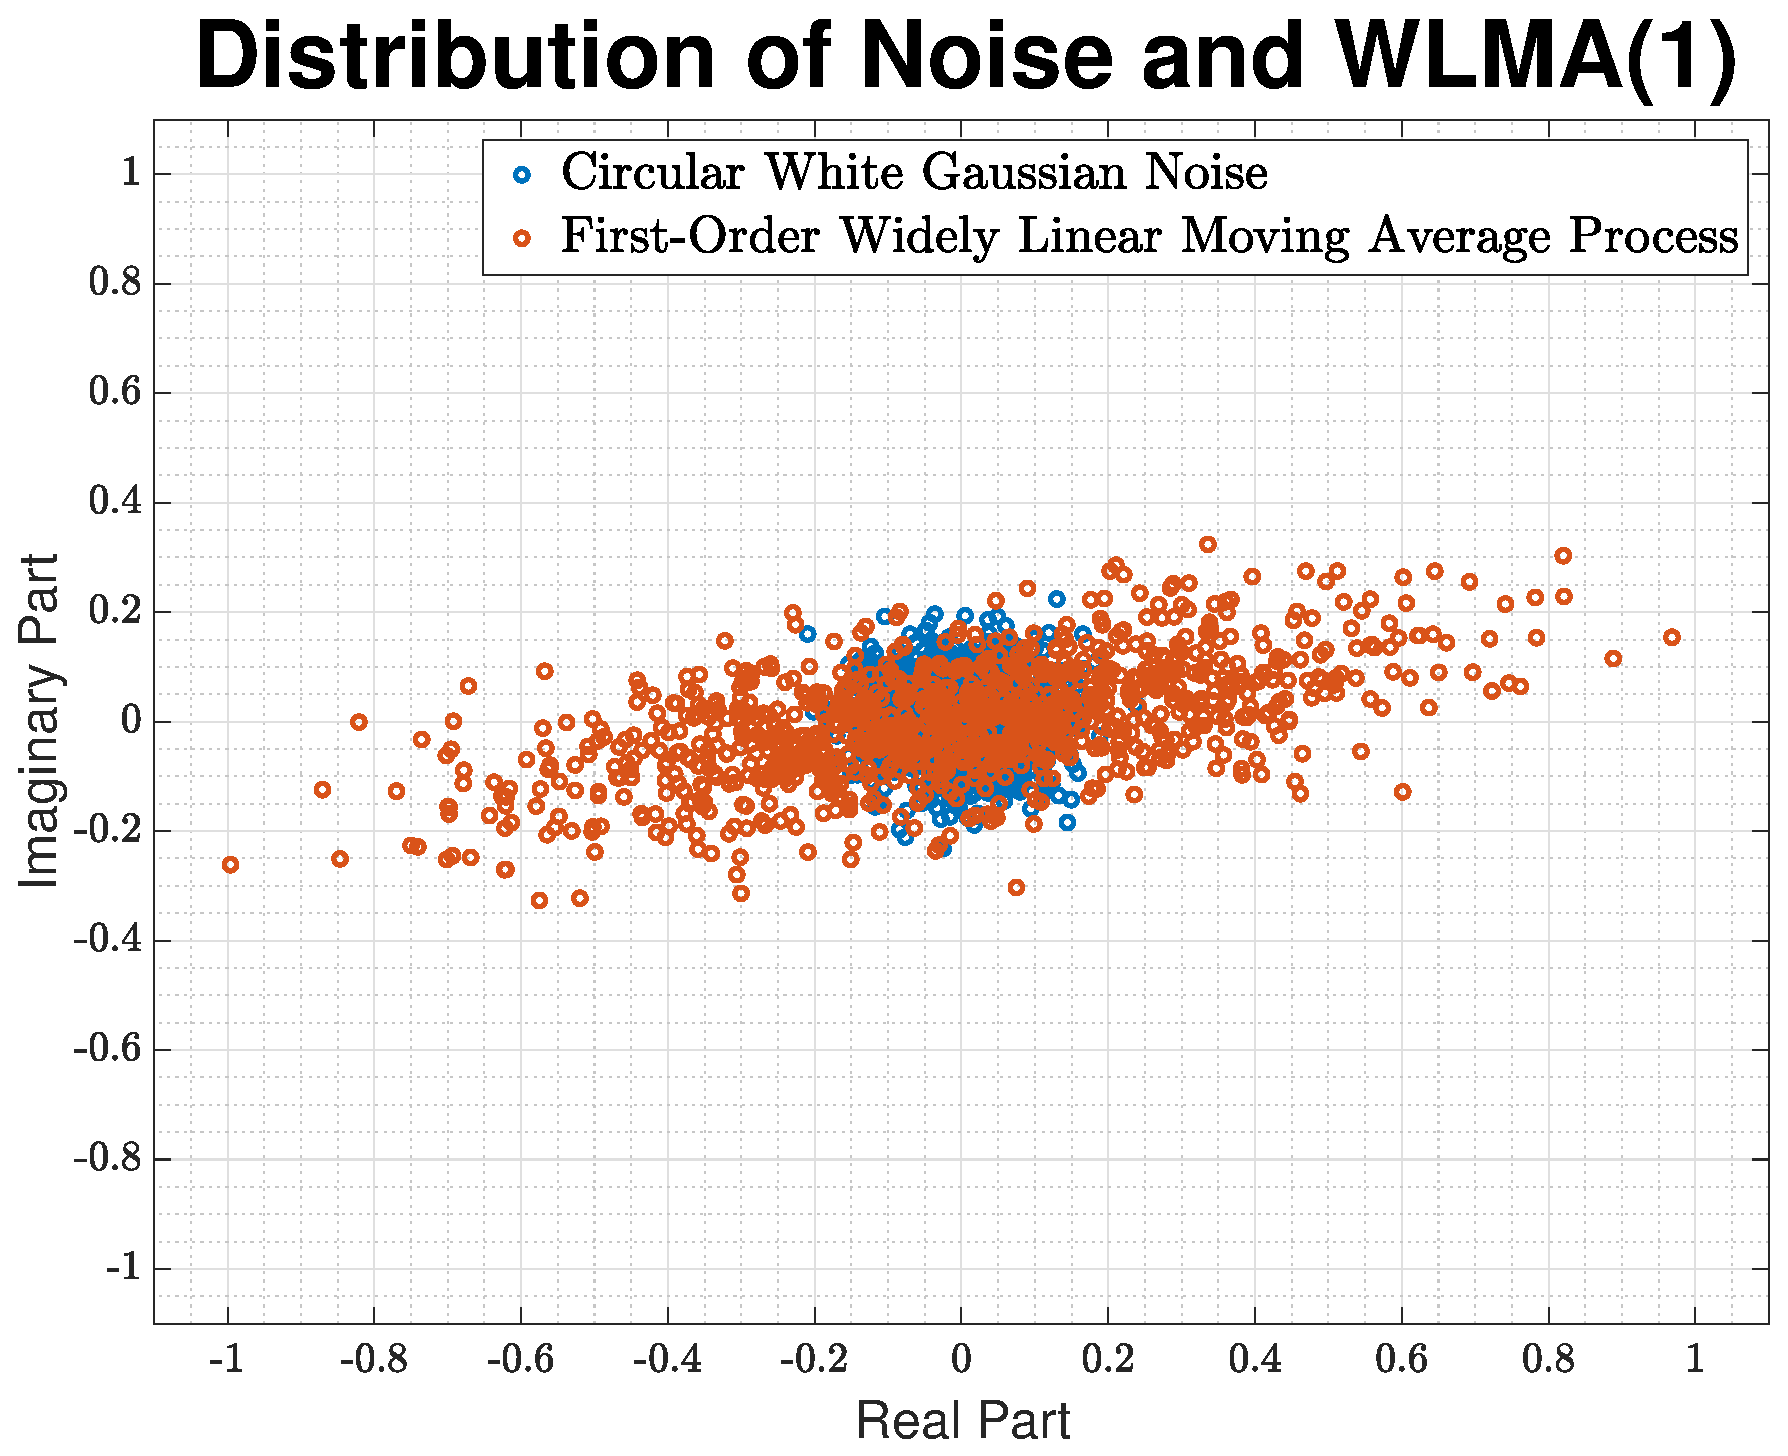
\includegraphics[width=0.32\textwidth]{part4/distributions}
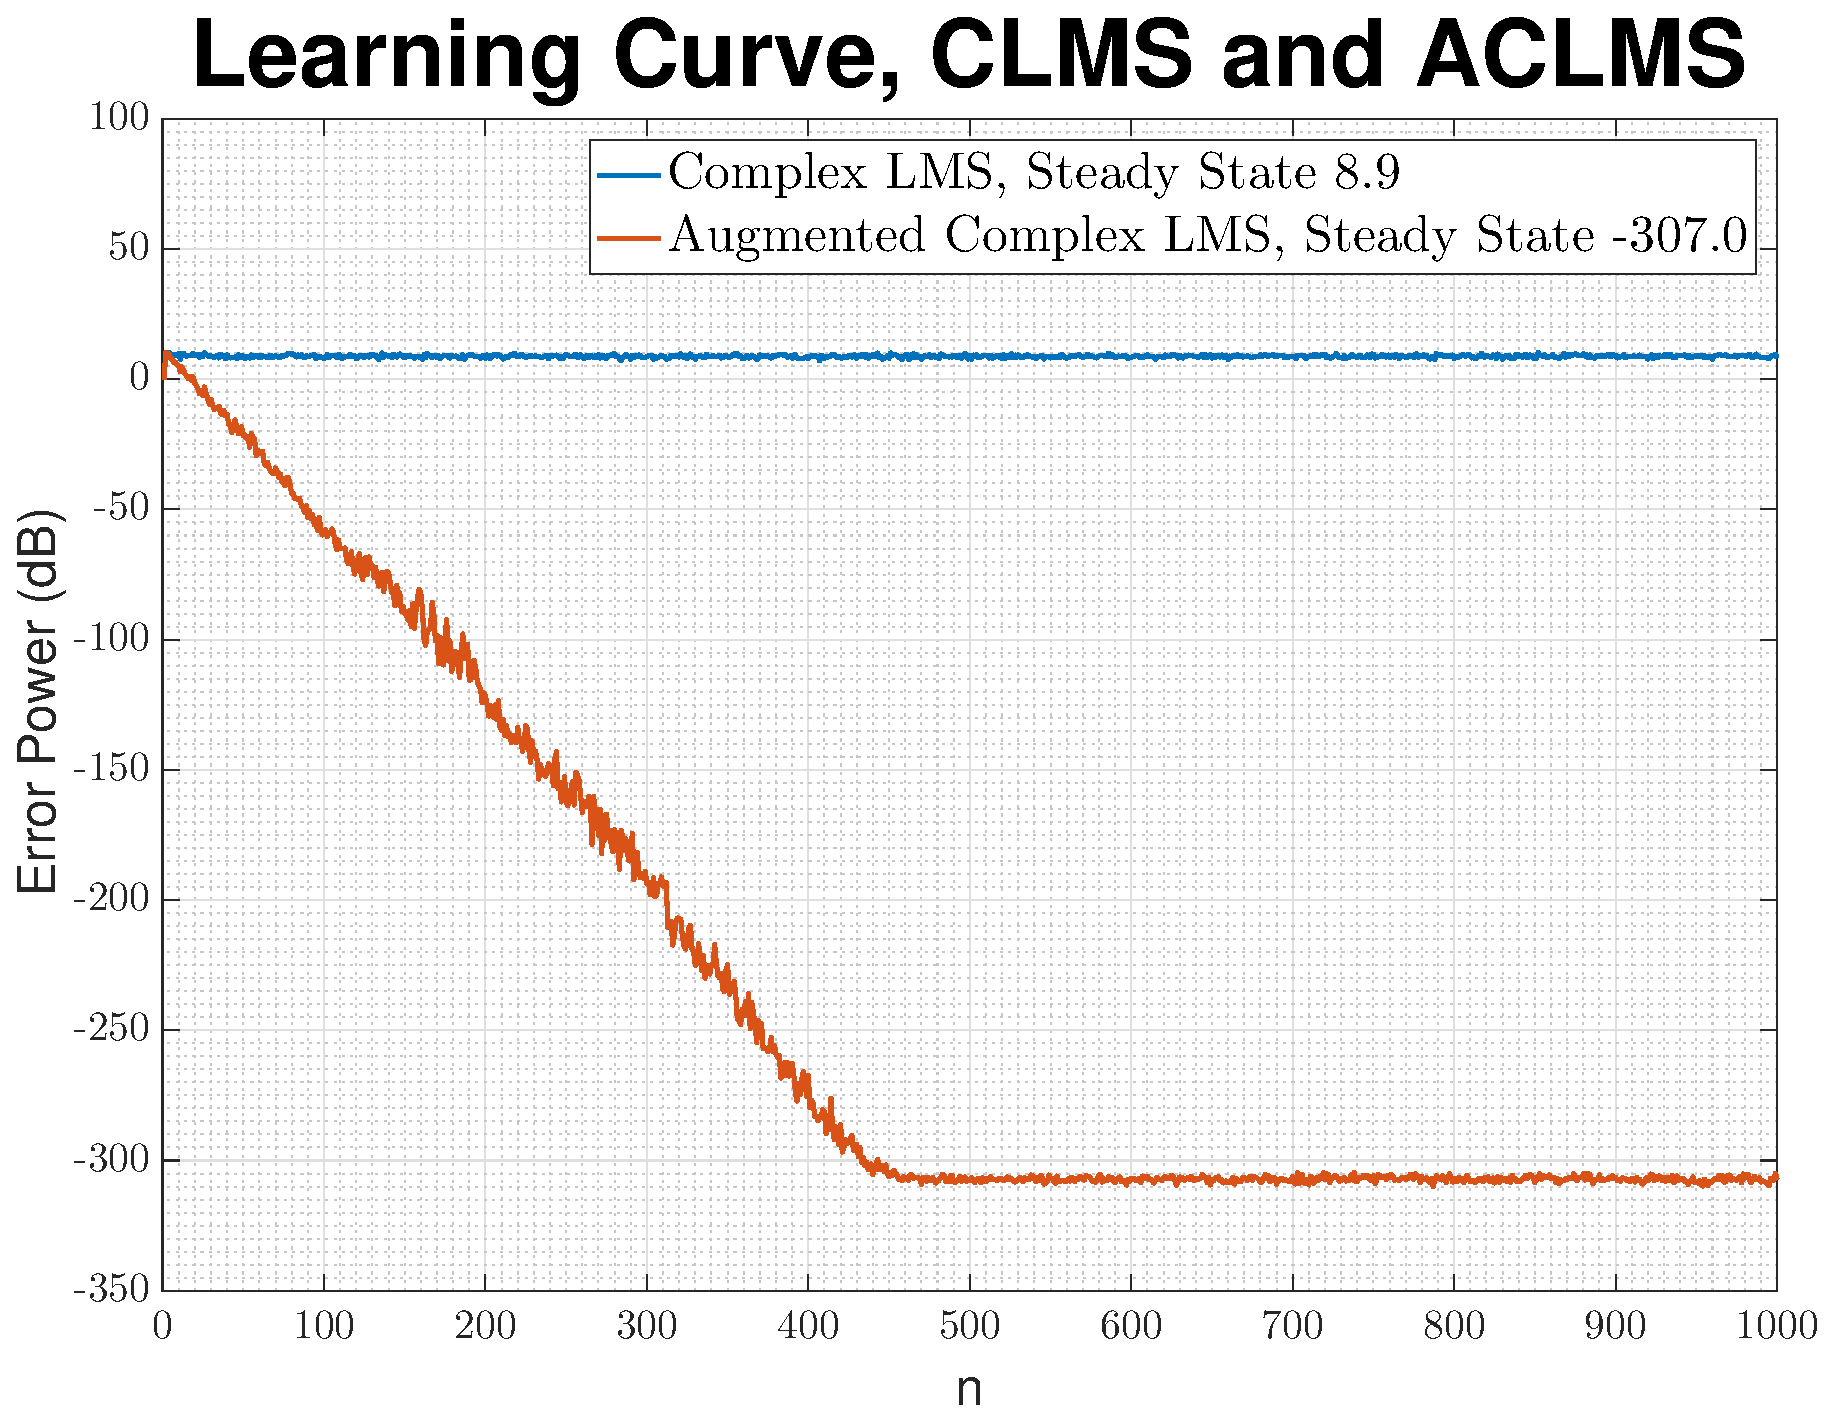
\includegraphics[width=0.32\textwidth]{part4/learning_curves_clms_aclms}
\caption{Comparison of Learning Curves using CLMS and ACLMS on Non-Circular WLMA(1) Process}
\end{figure}

\begin{figure}[H]
\centering{}
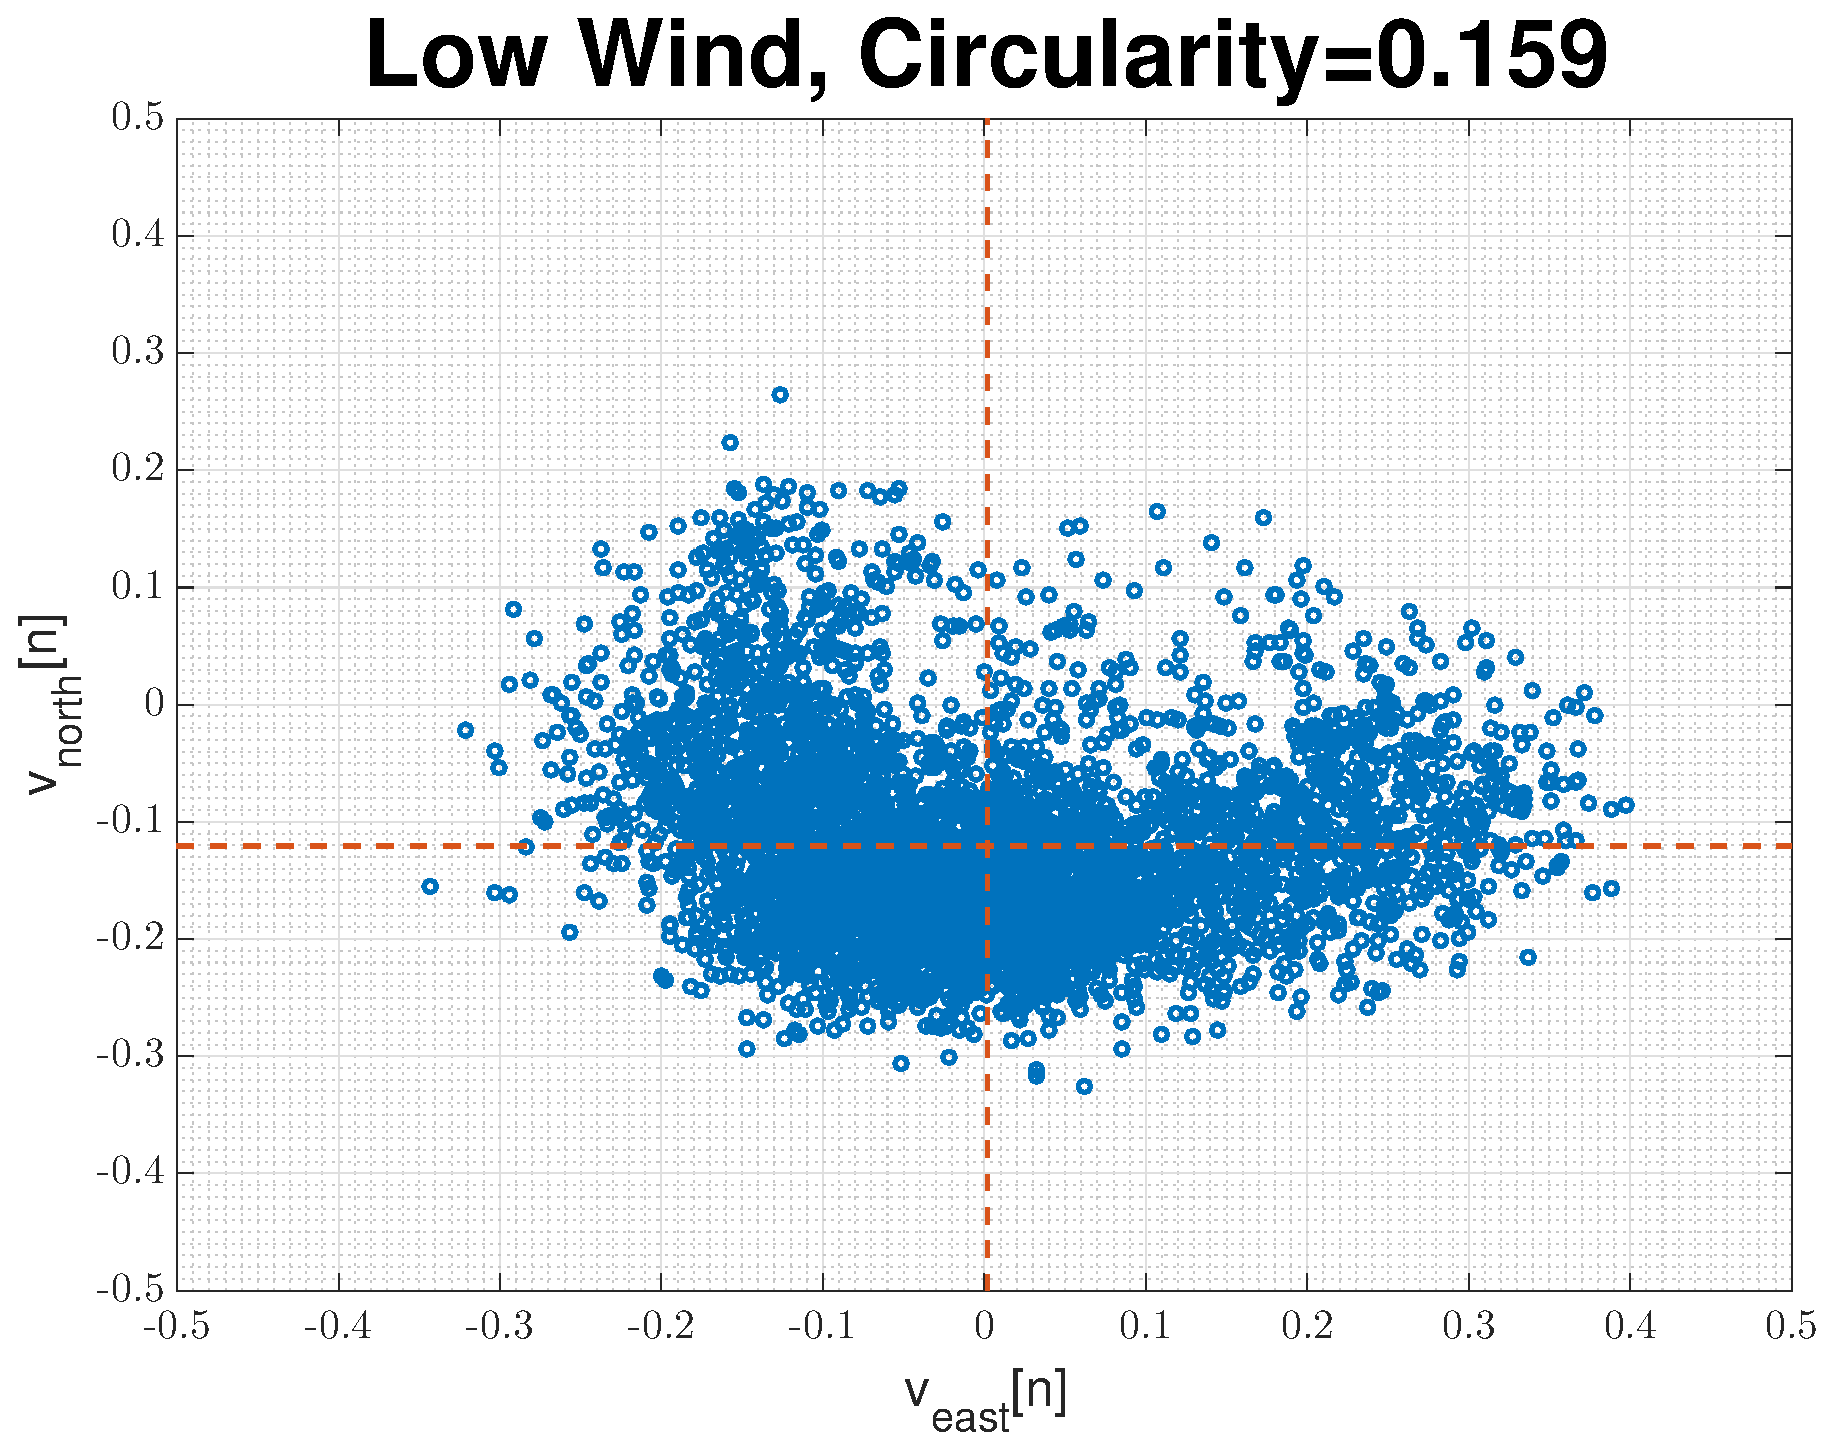
\includegraphics[width=0.32\textwidth]{part4/circularity_low_wind}
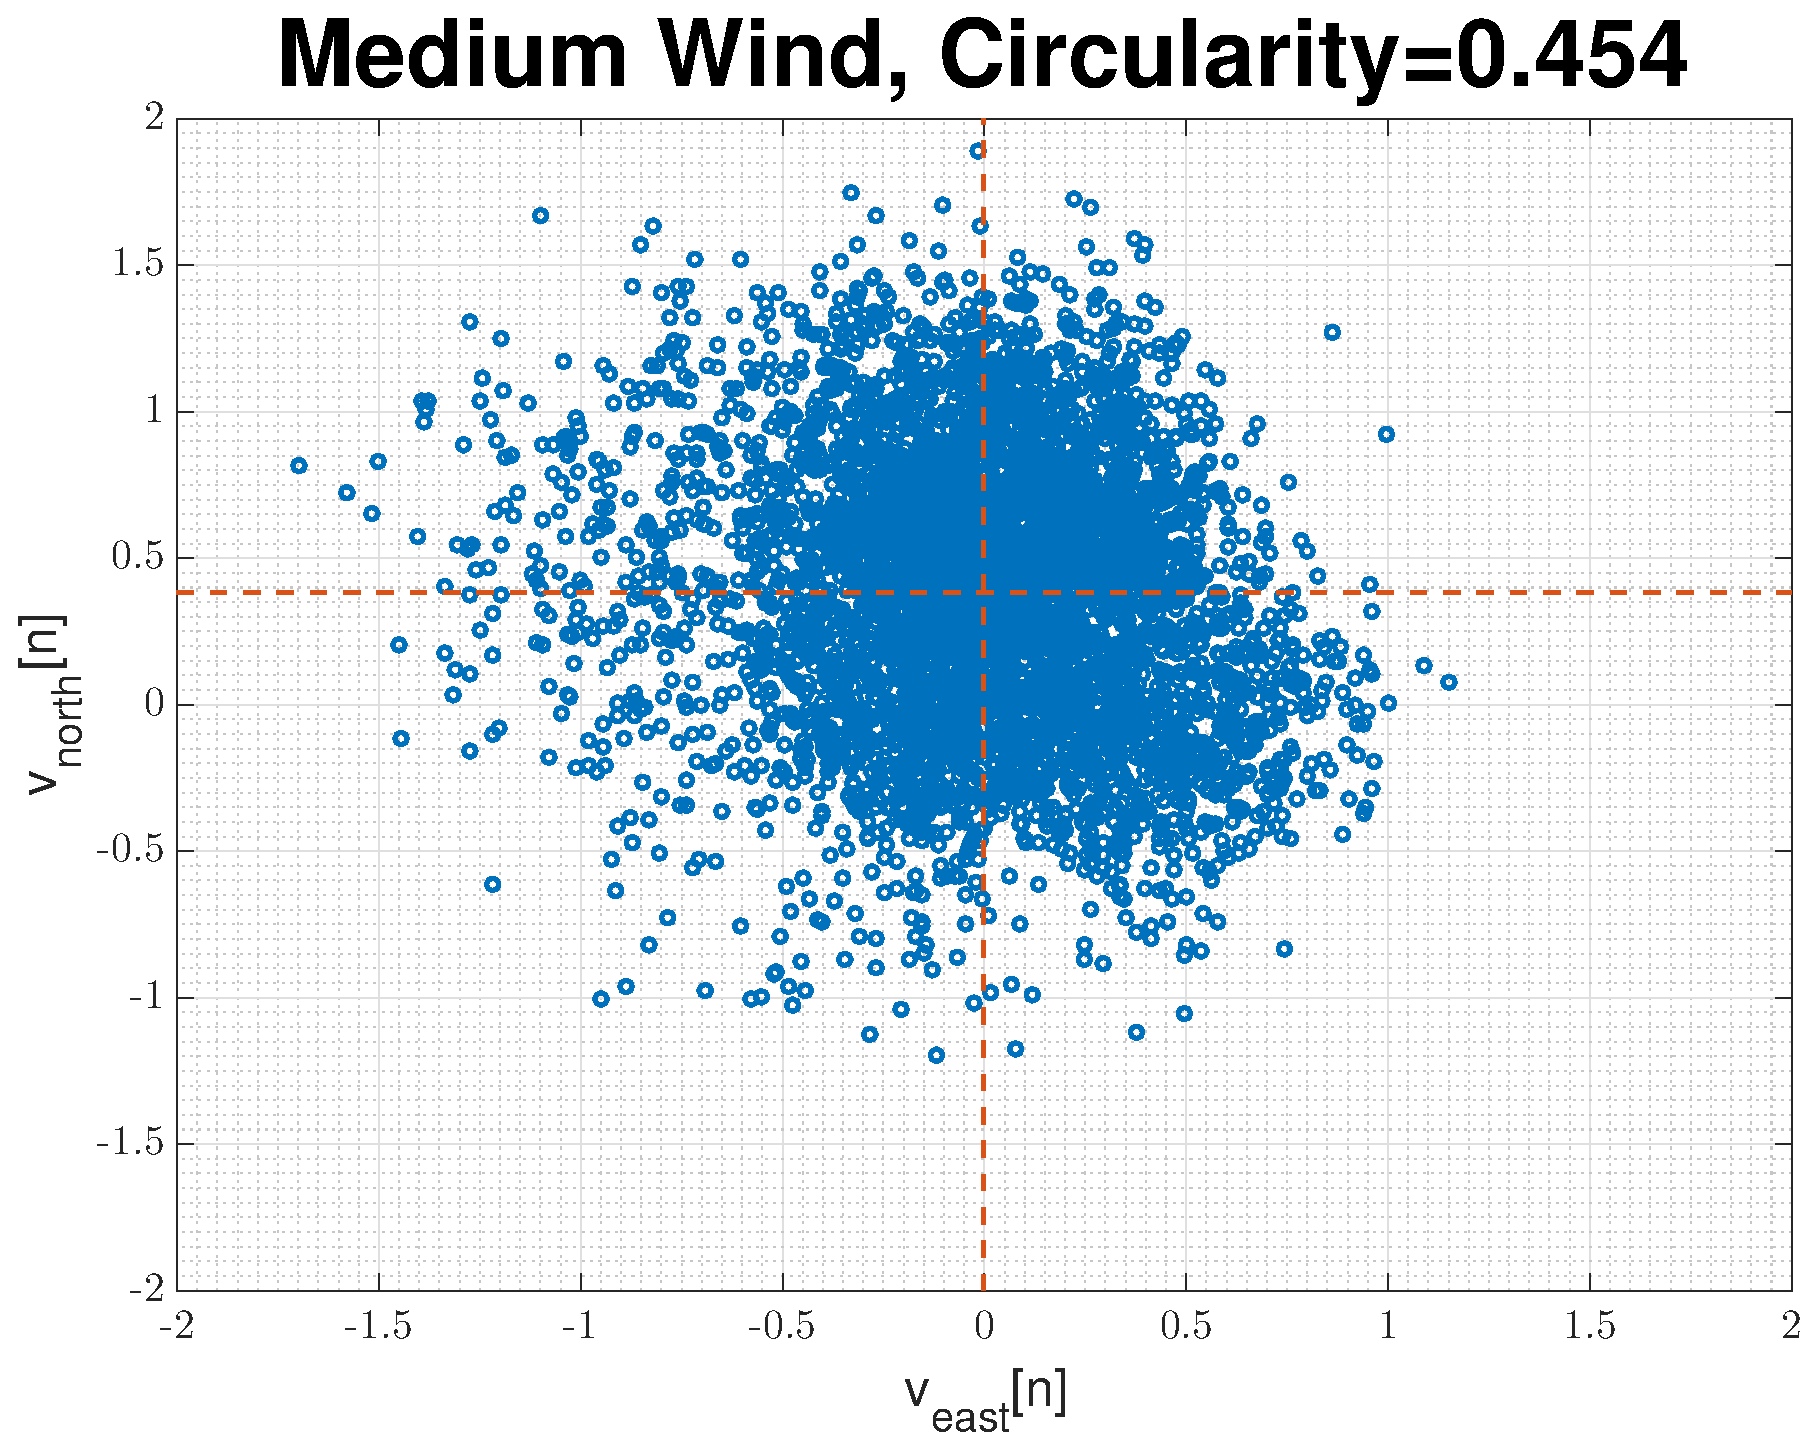
\includegraphics[width=0.32\textwidth]{part4/circularity_medium_wind}
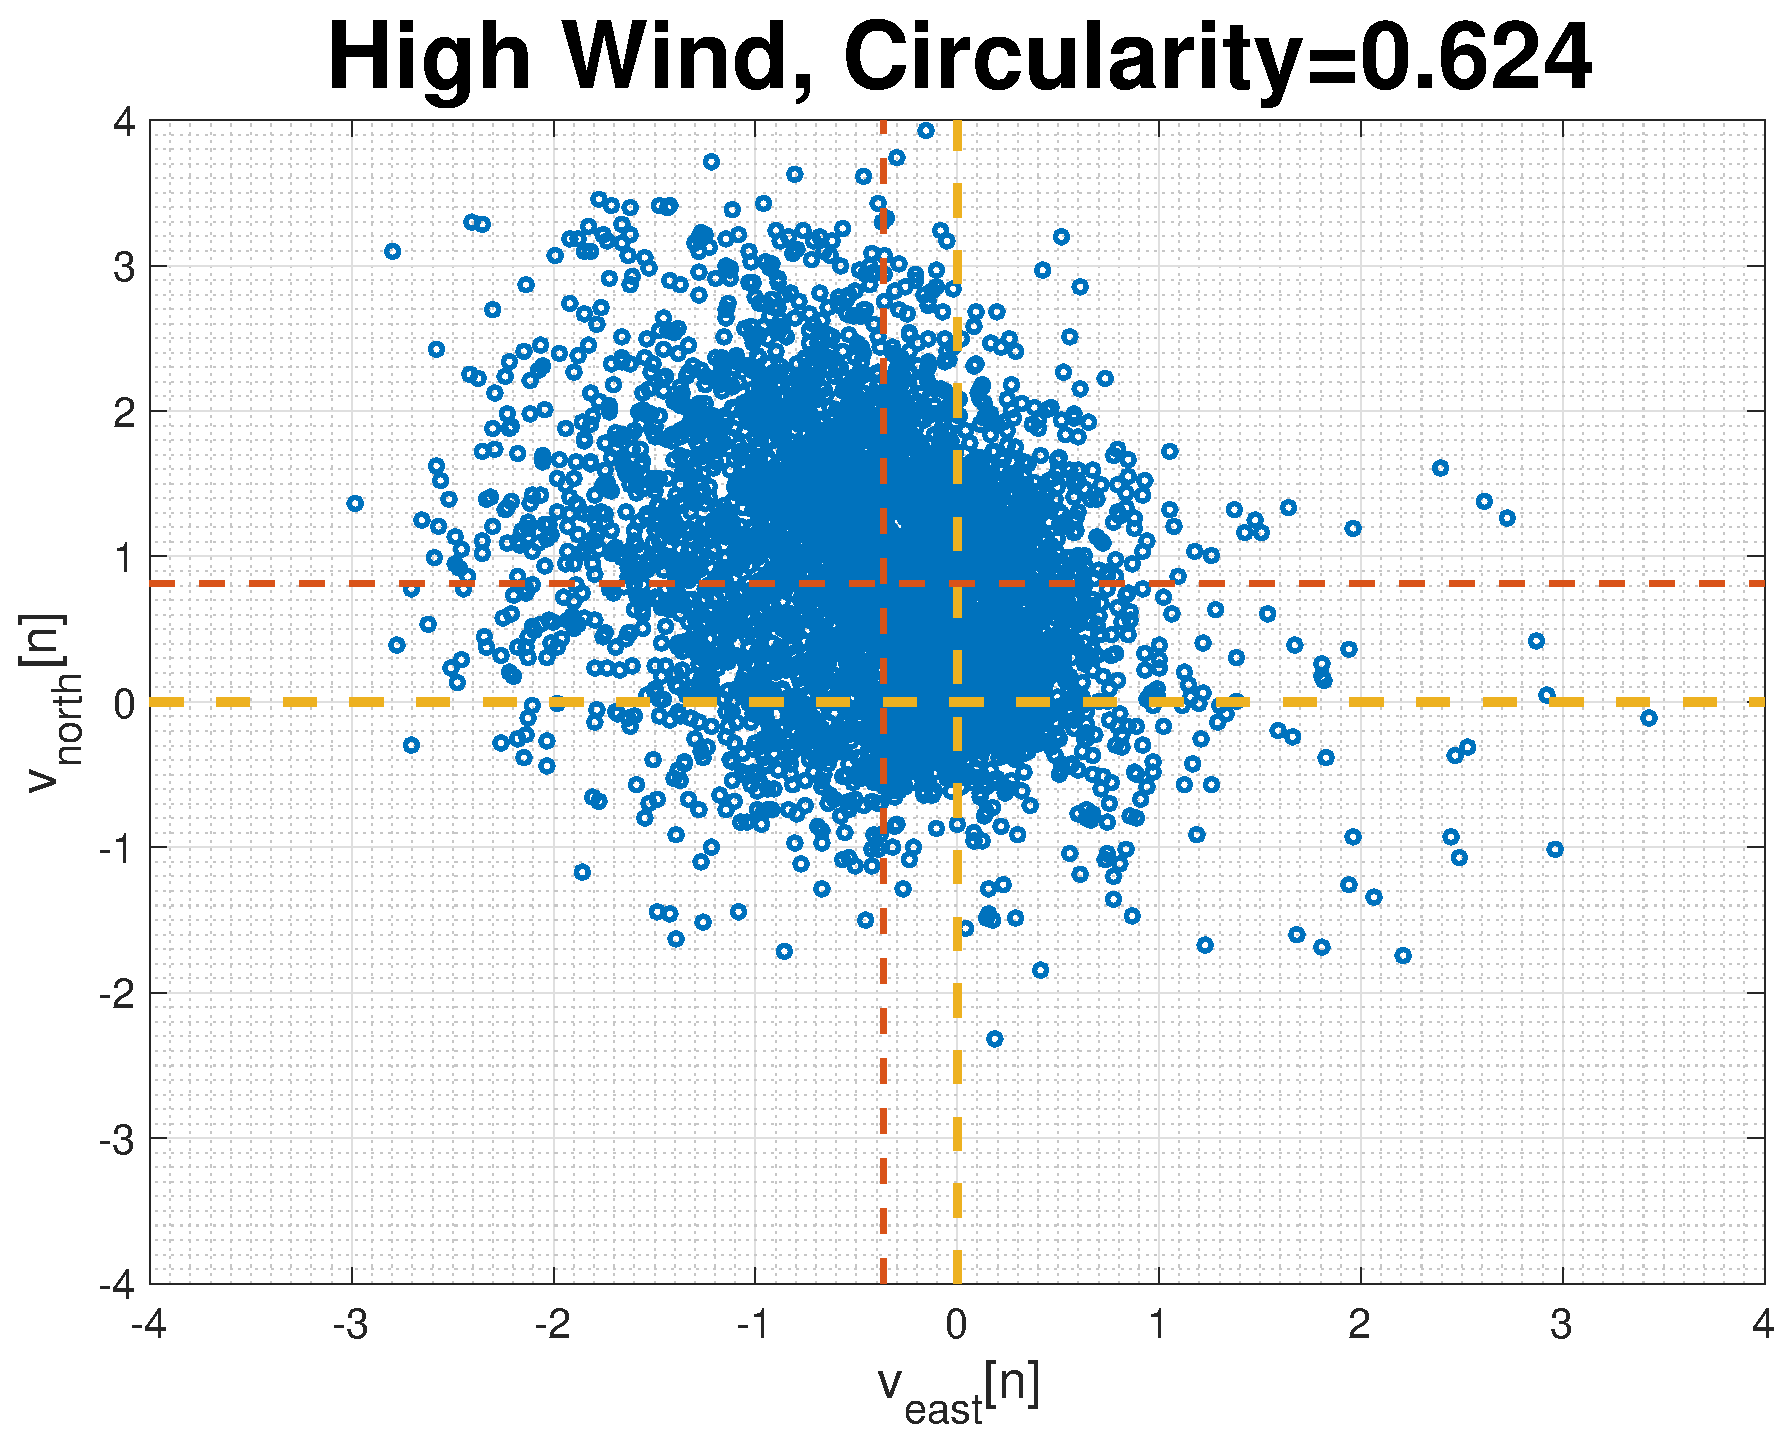
\includegraphics[width=0.32\textwidth]{part4/circularity_high_wind}
\caption{Circularity Plots for Different Wind Speeds}
\end{figure}


\begin{figure}[H]
\centering{}
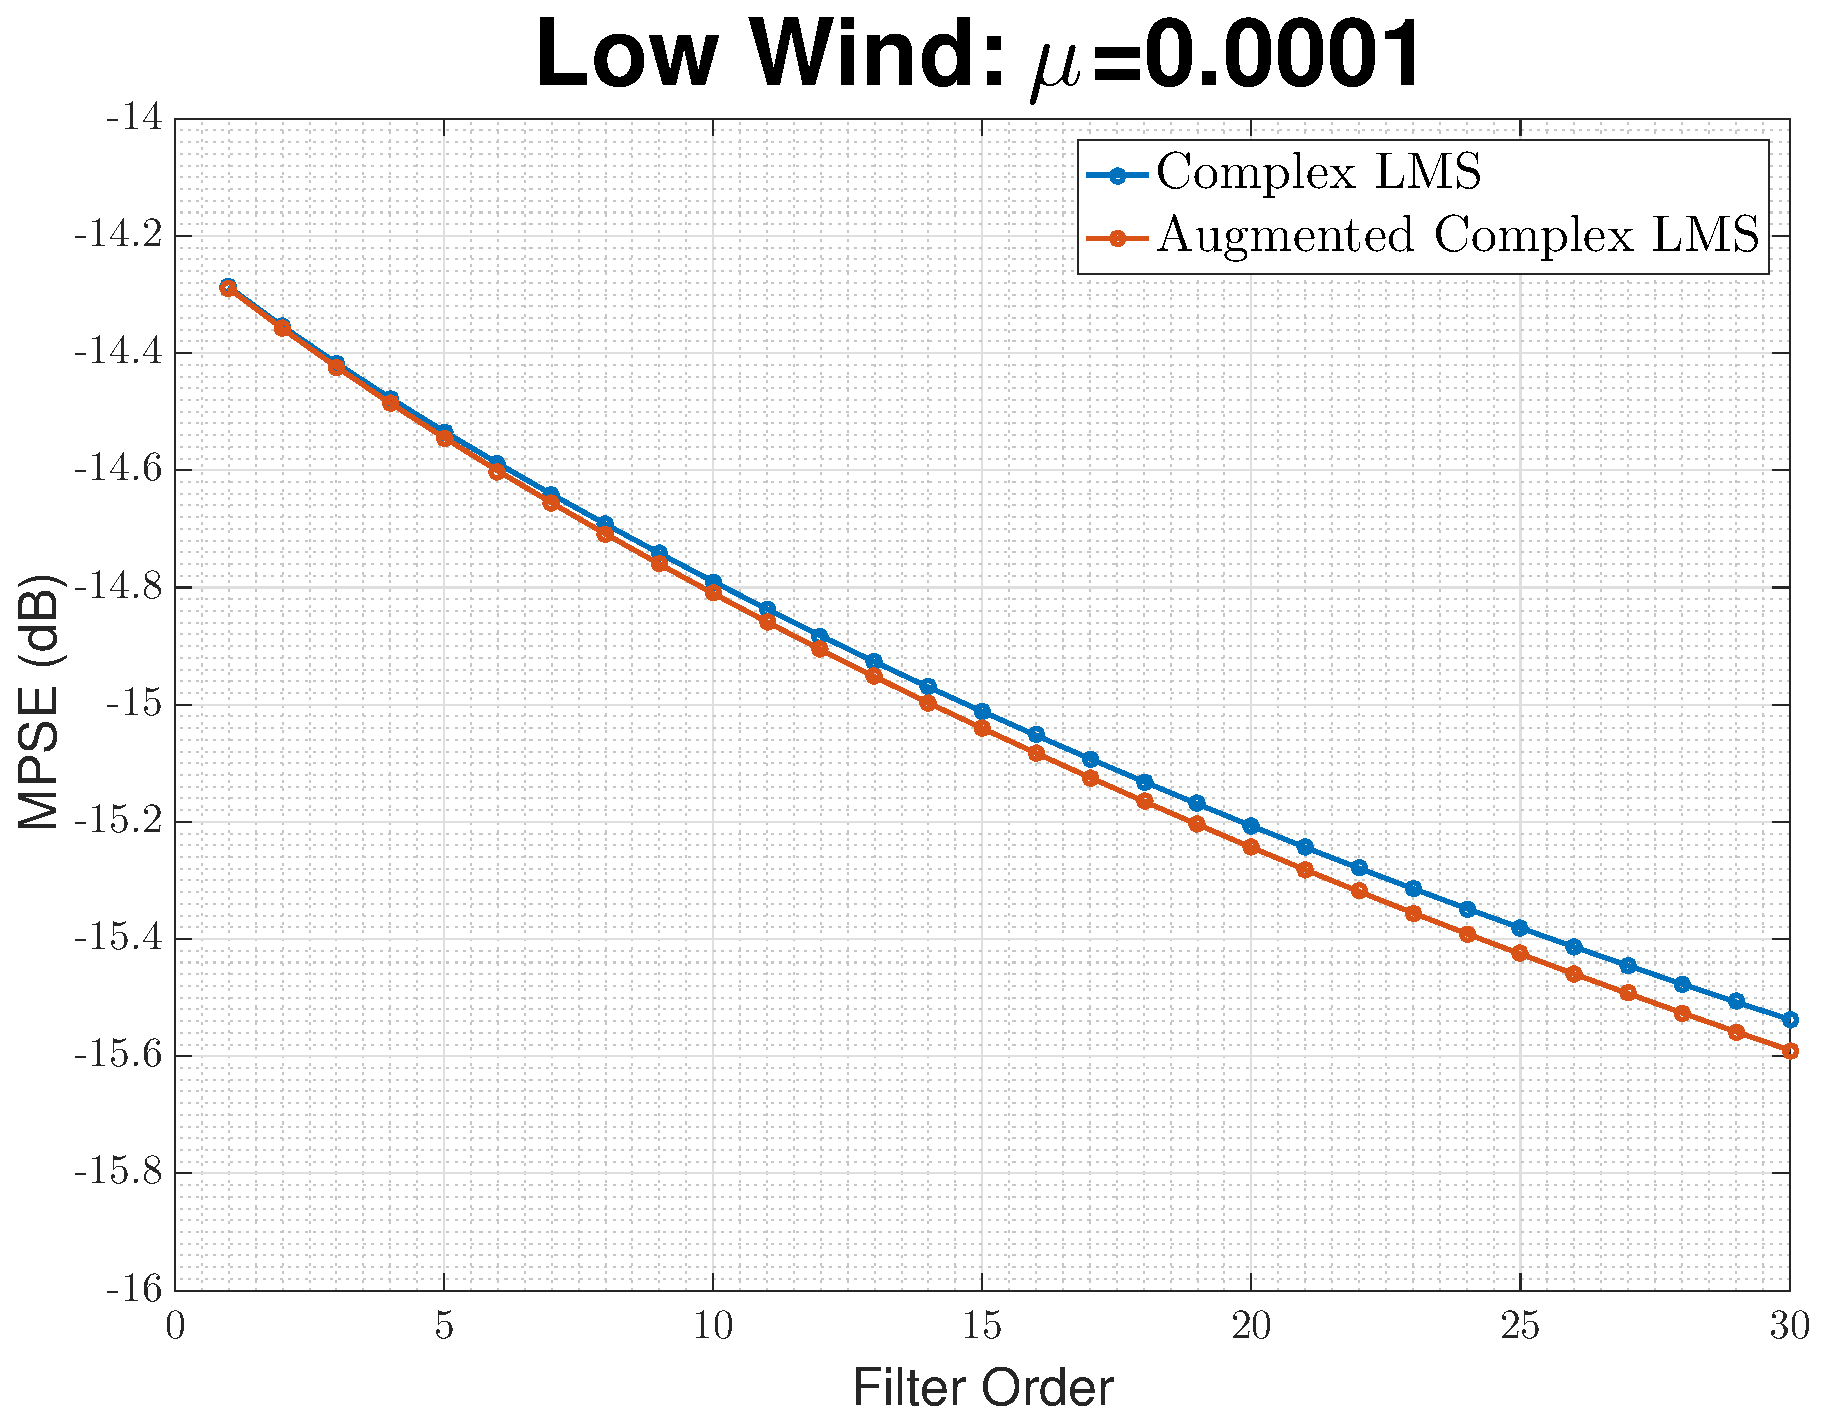
\includegraphics[width=0.32\textwidth]{part4/filt_order_low_wind}
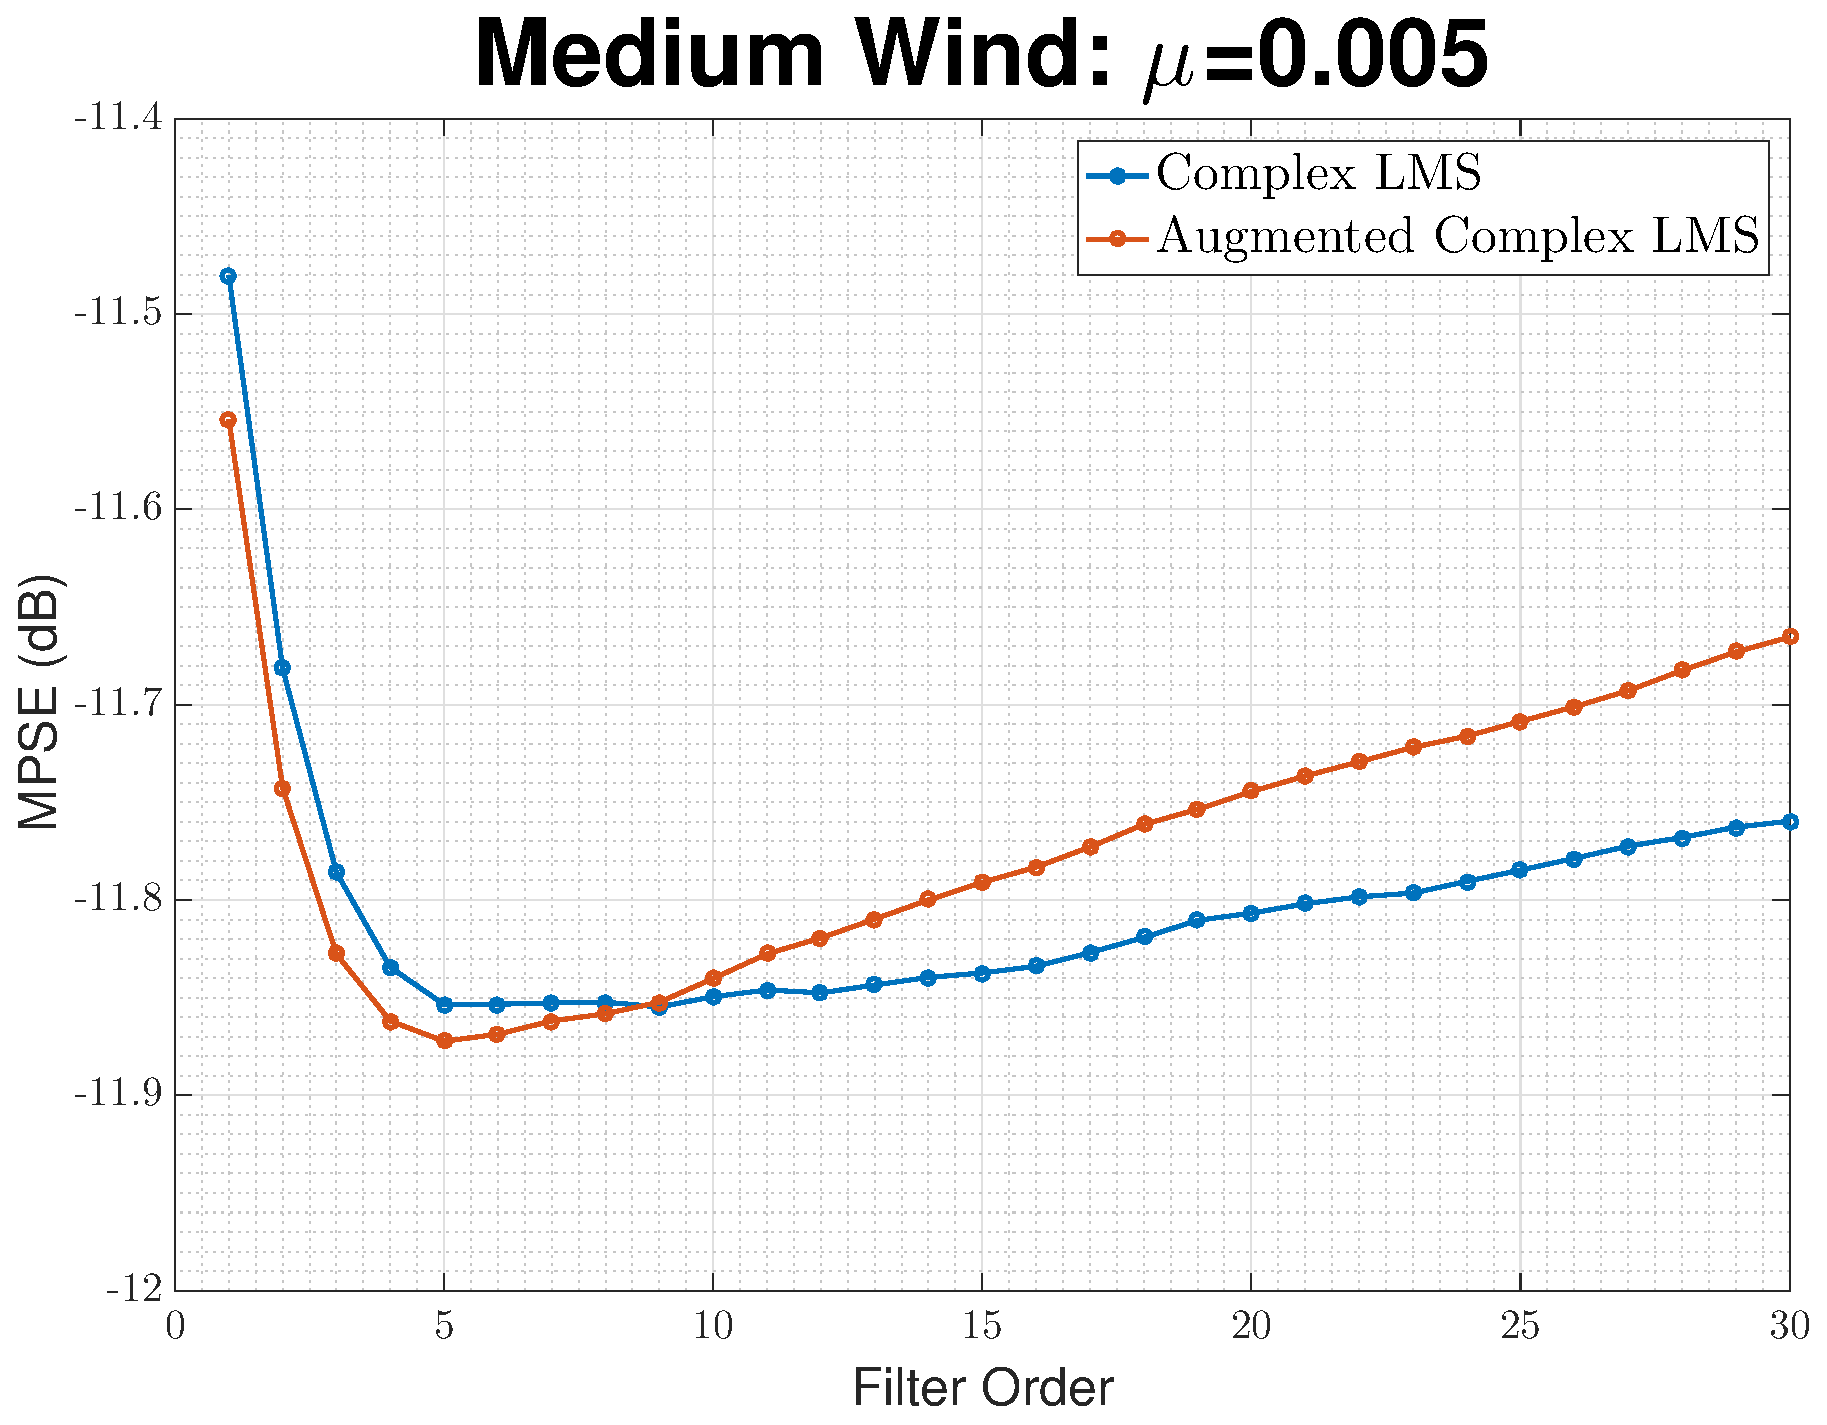
\includegraphics[width=0.32\textwidth]{part4/filt_order_medium_wind}
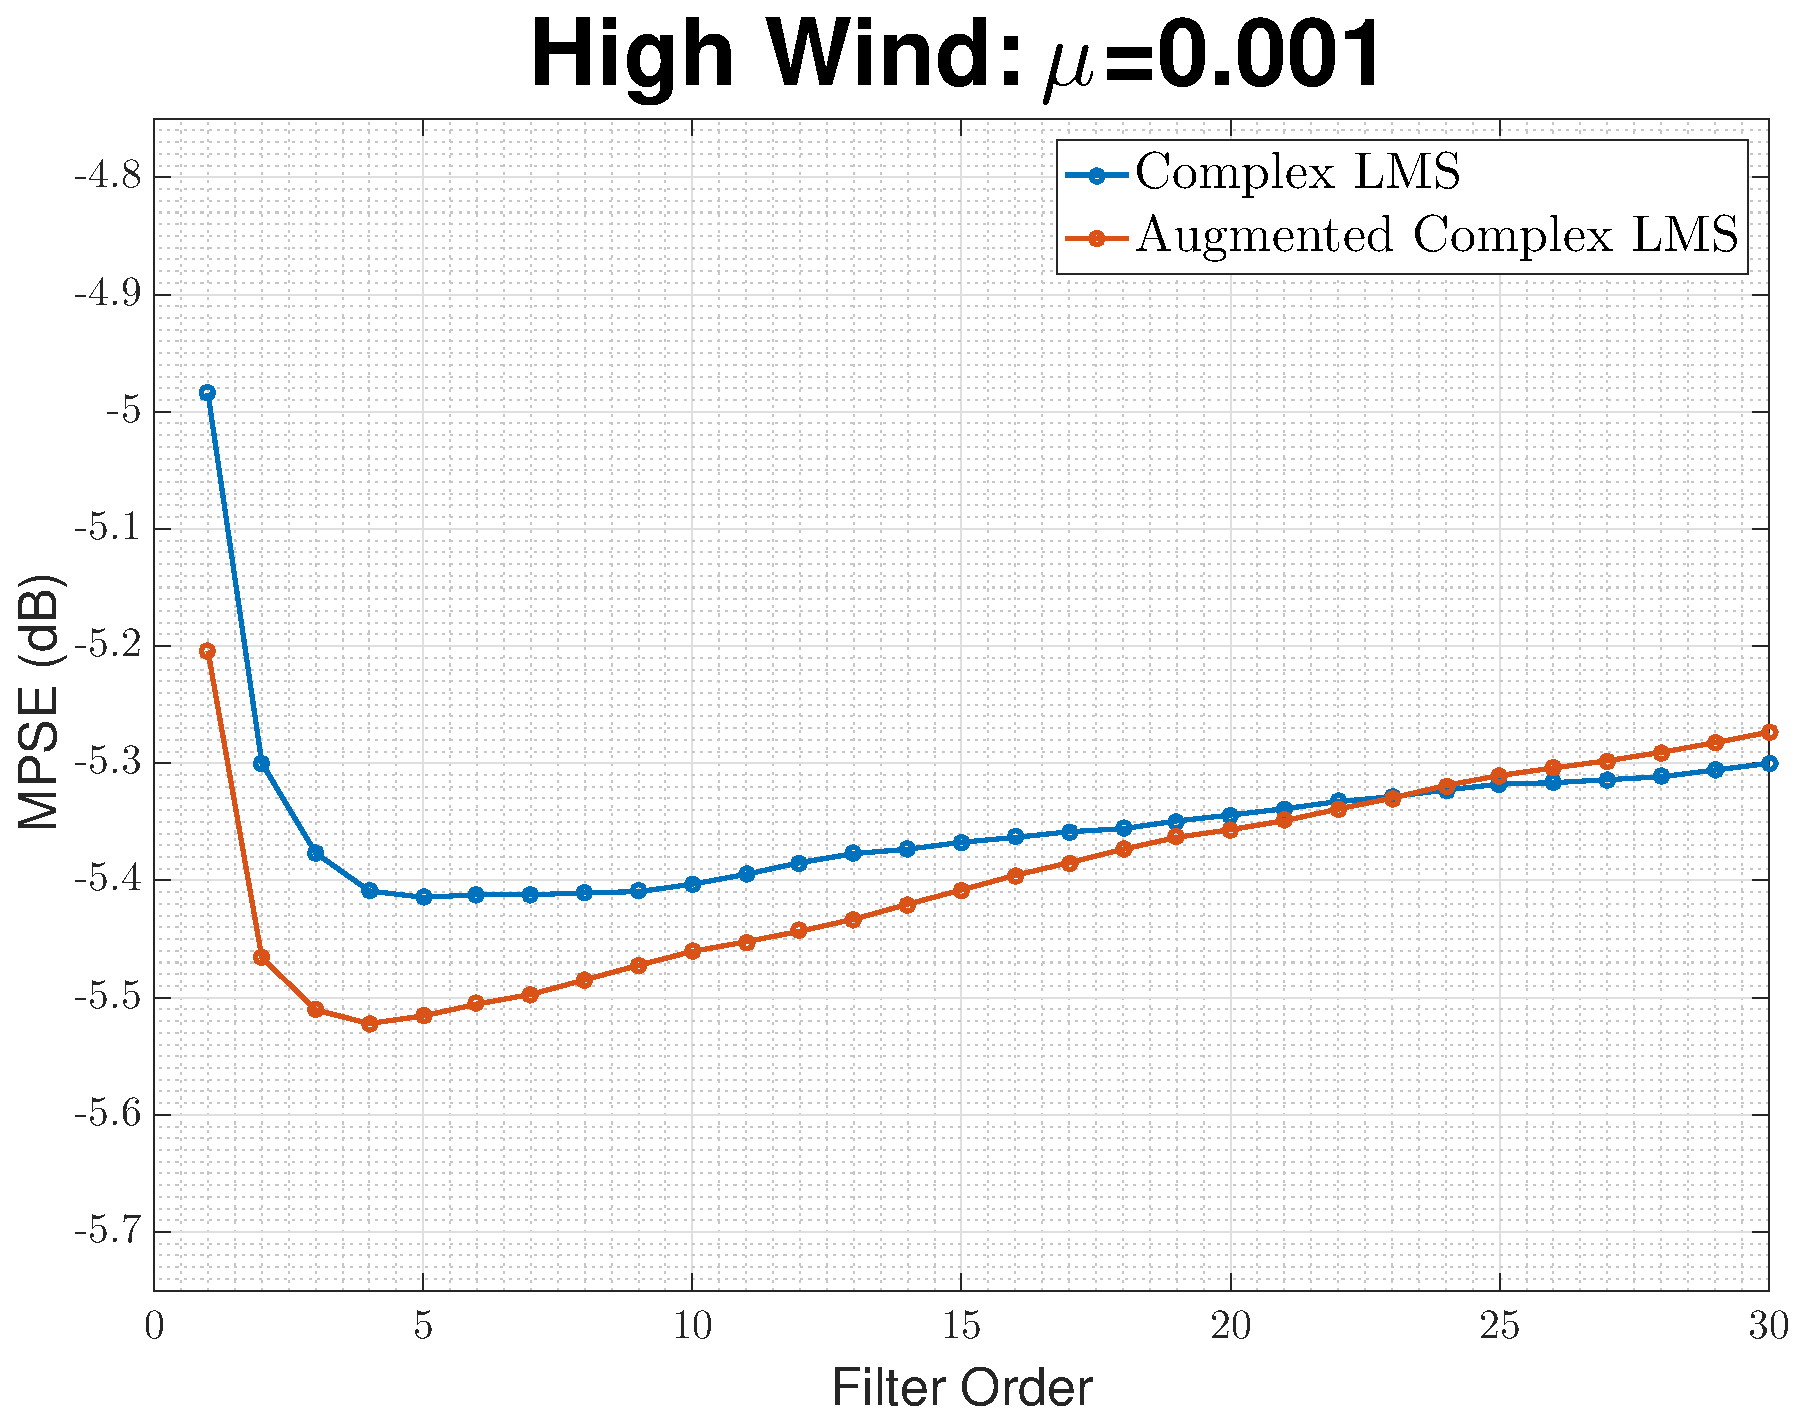
\includegraphics[width=0.32\textwidth]{part4/filt_order_high_wind}
\caption{Scaling of MPSE with Increase in Filter Order}
\end{figure}


\begin{figure}[H]
\centering{}
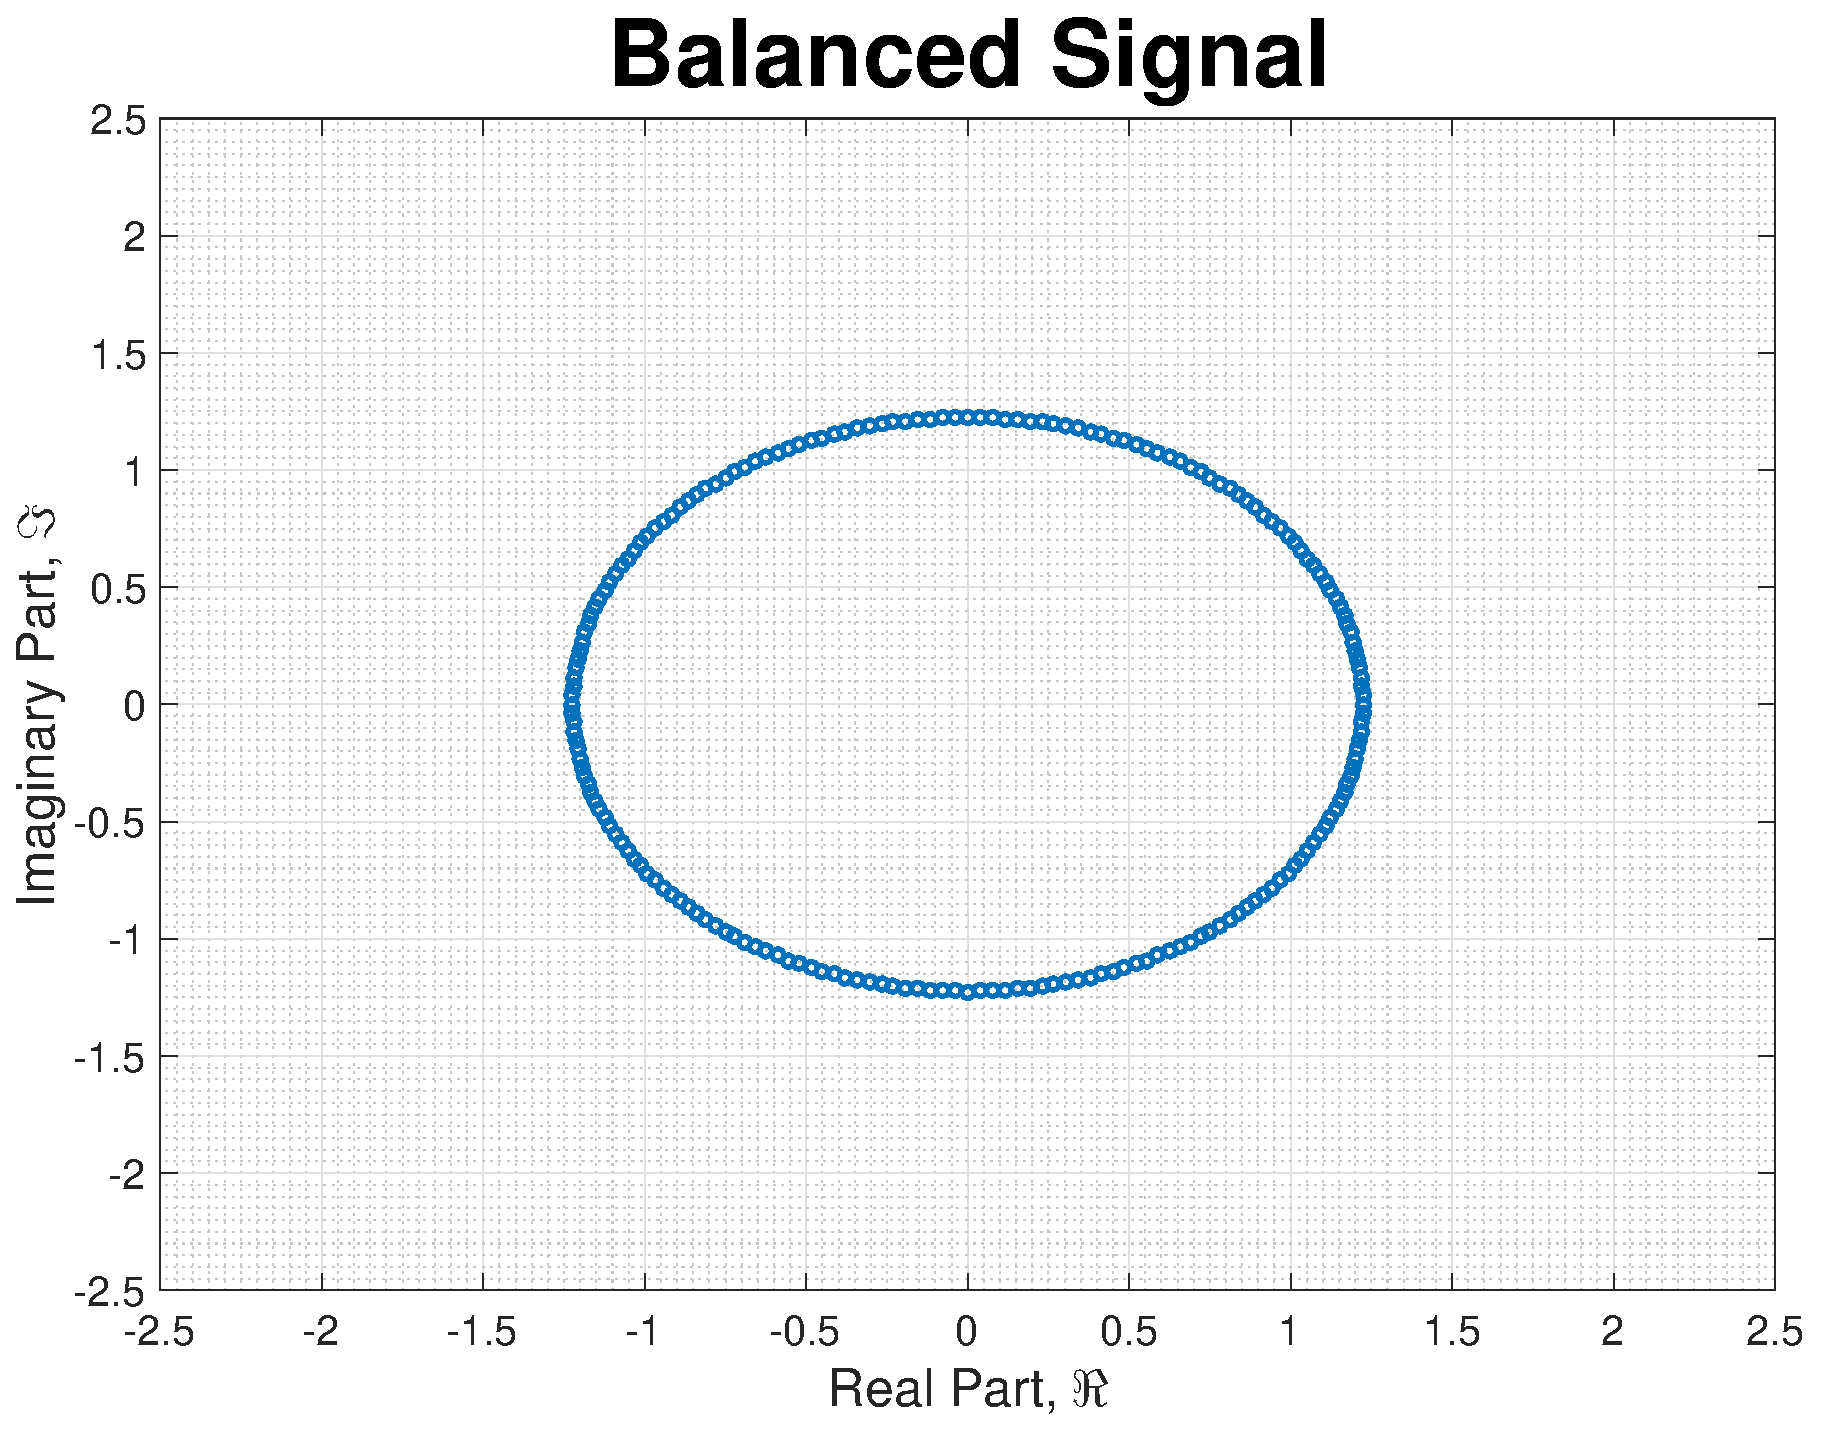
\includegraphics[width=0.32\textwidth]{part4/balanced_signal}
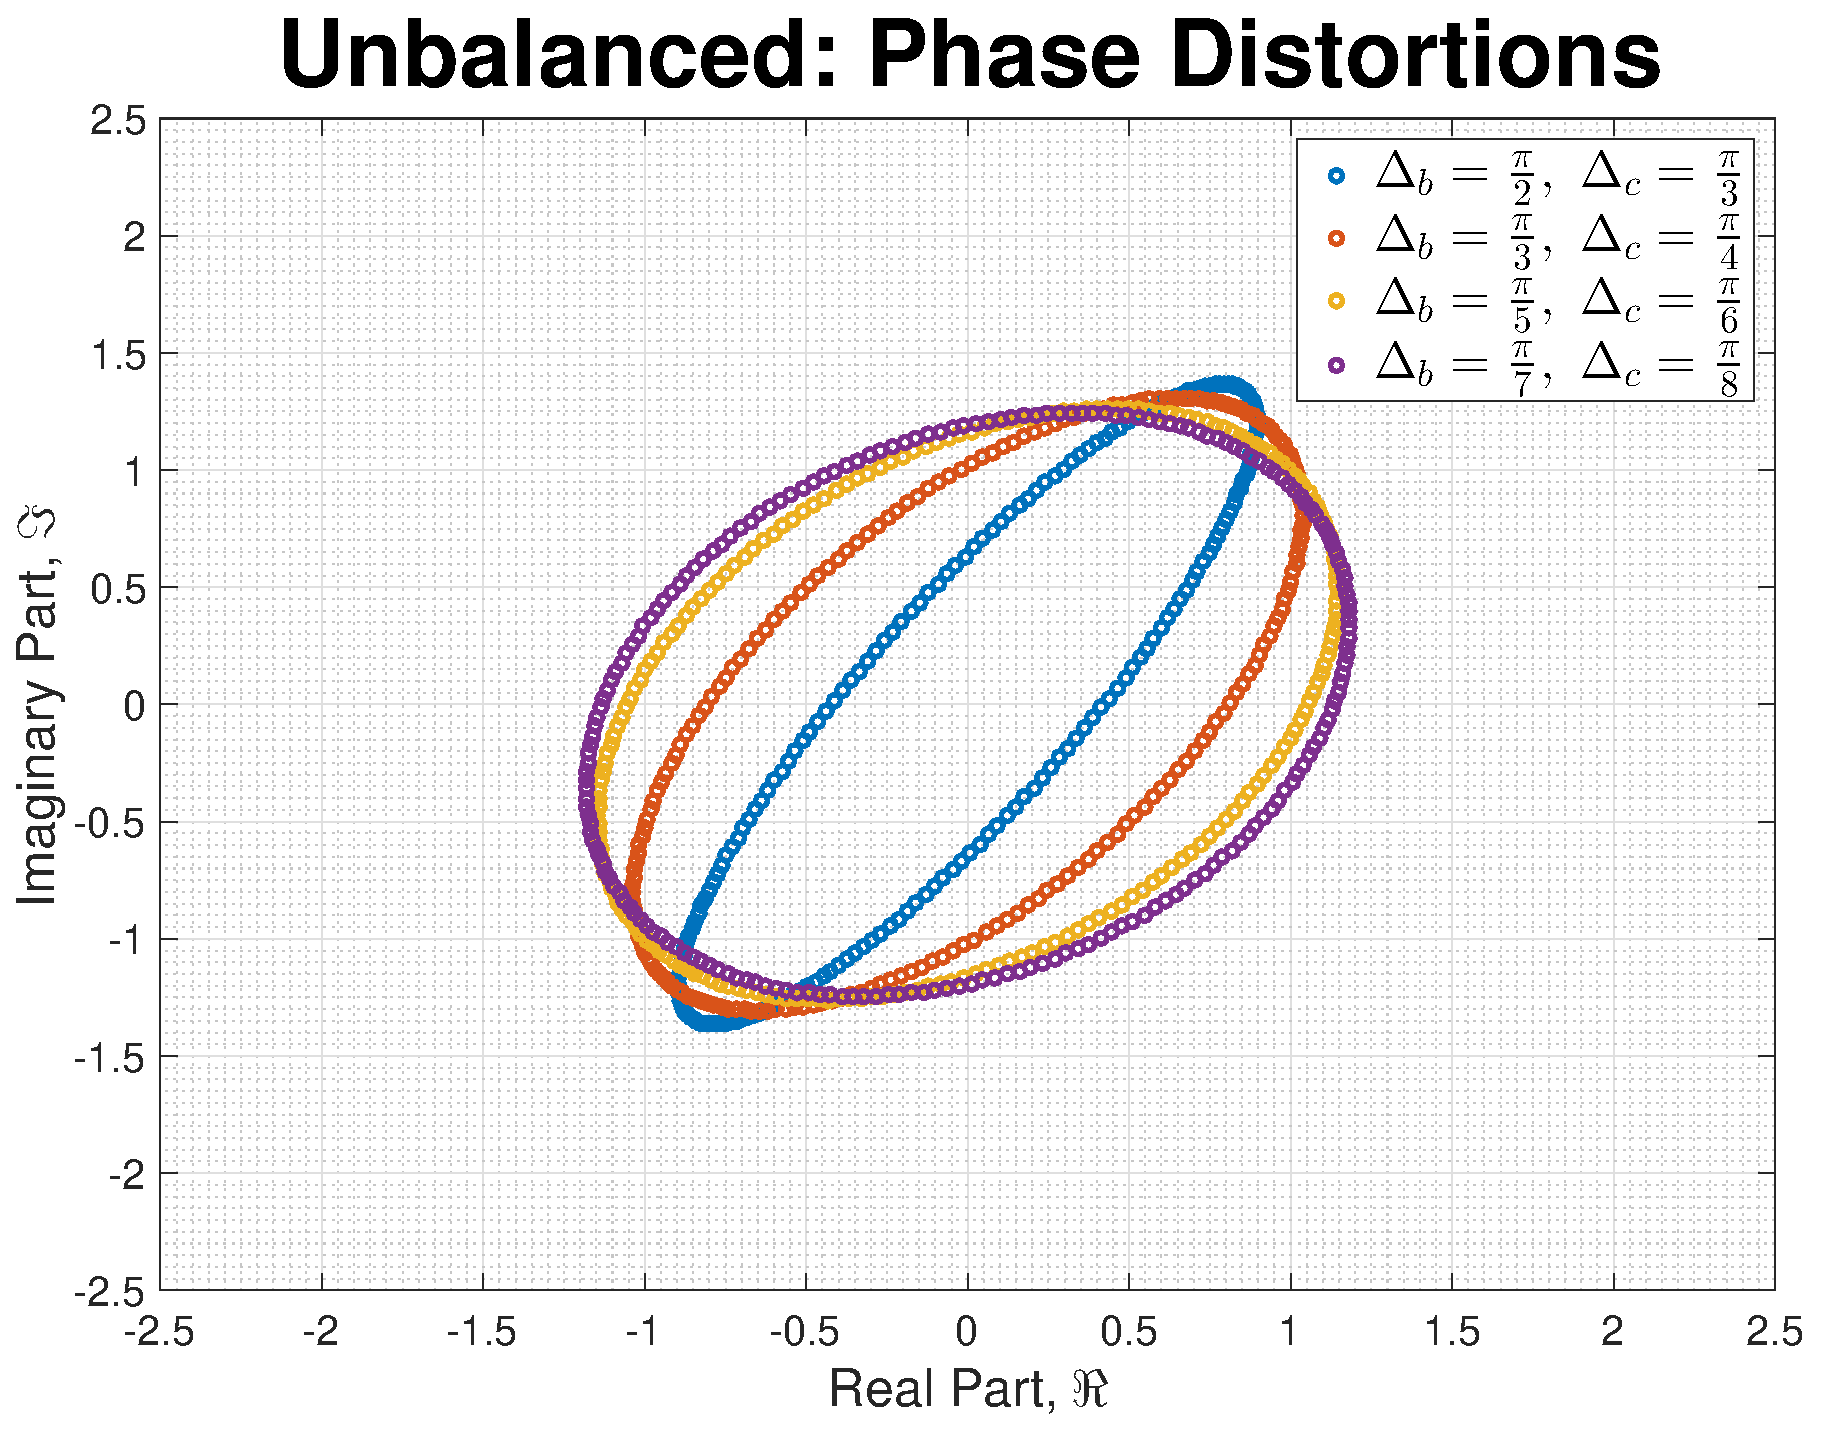
\includegraphics[width=0.32\textwidth]{part4/unbalanced_phase_distortion}
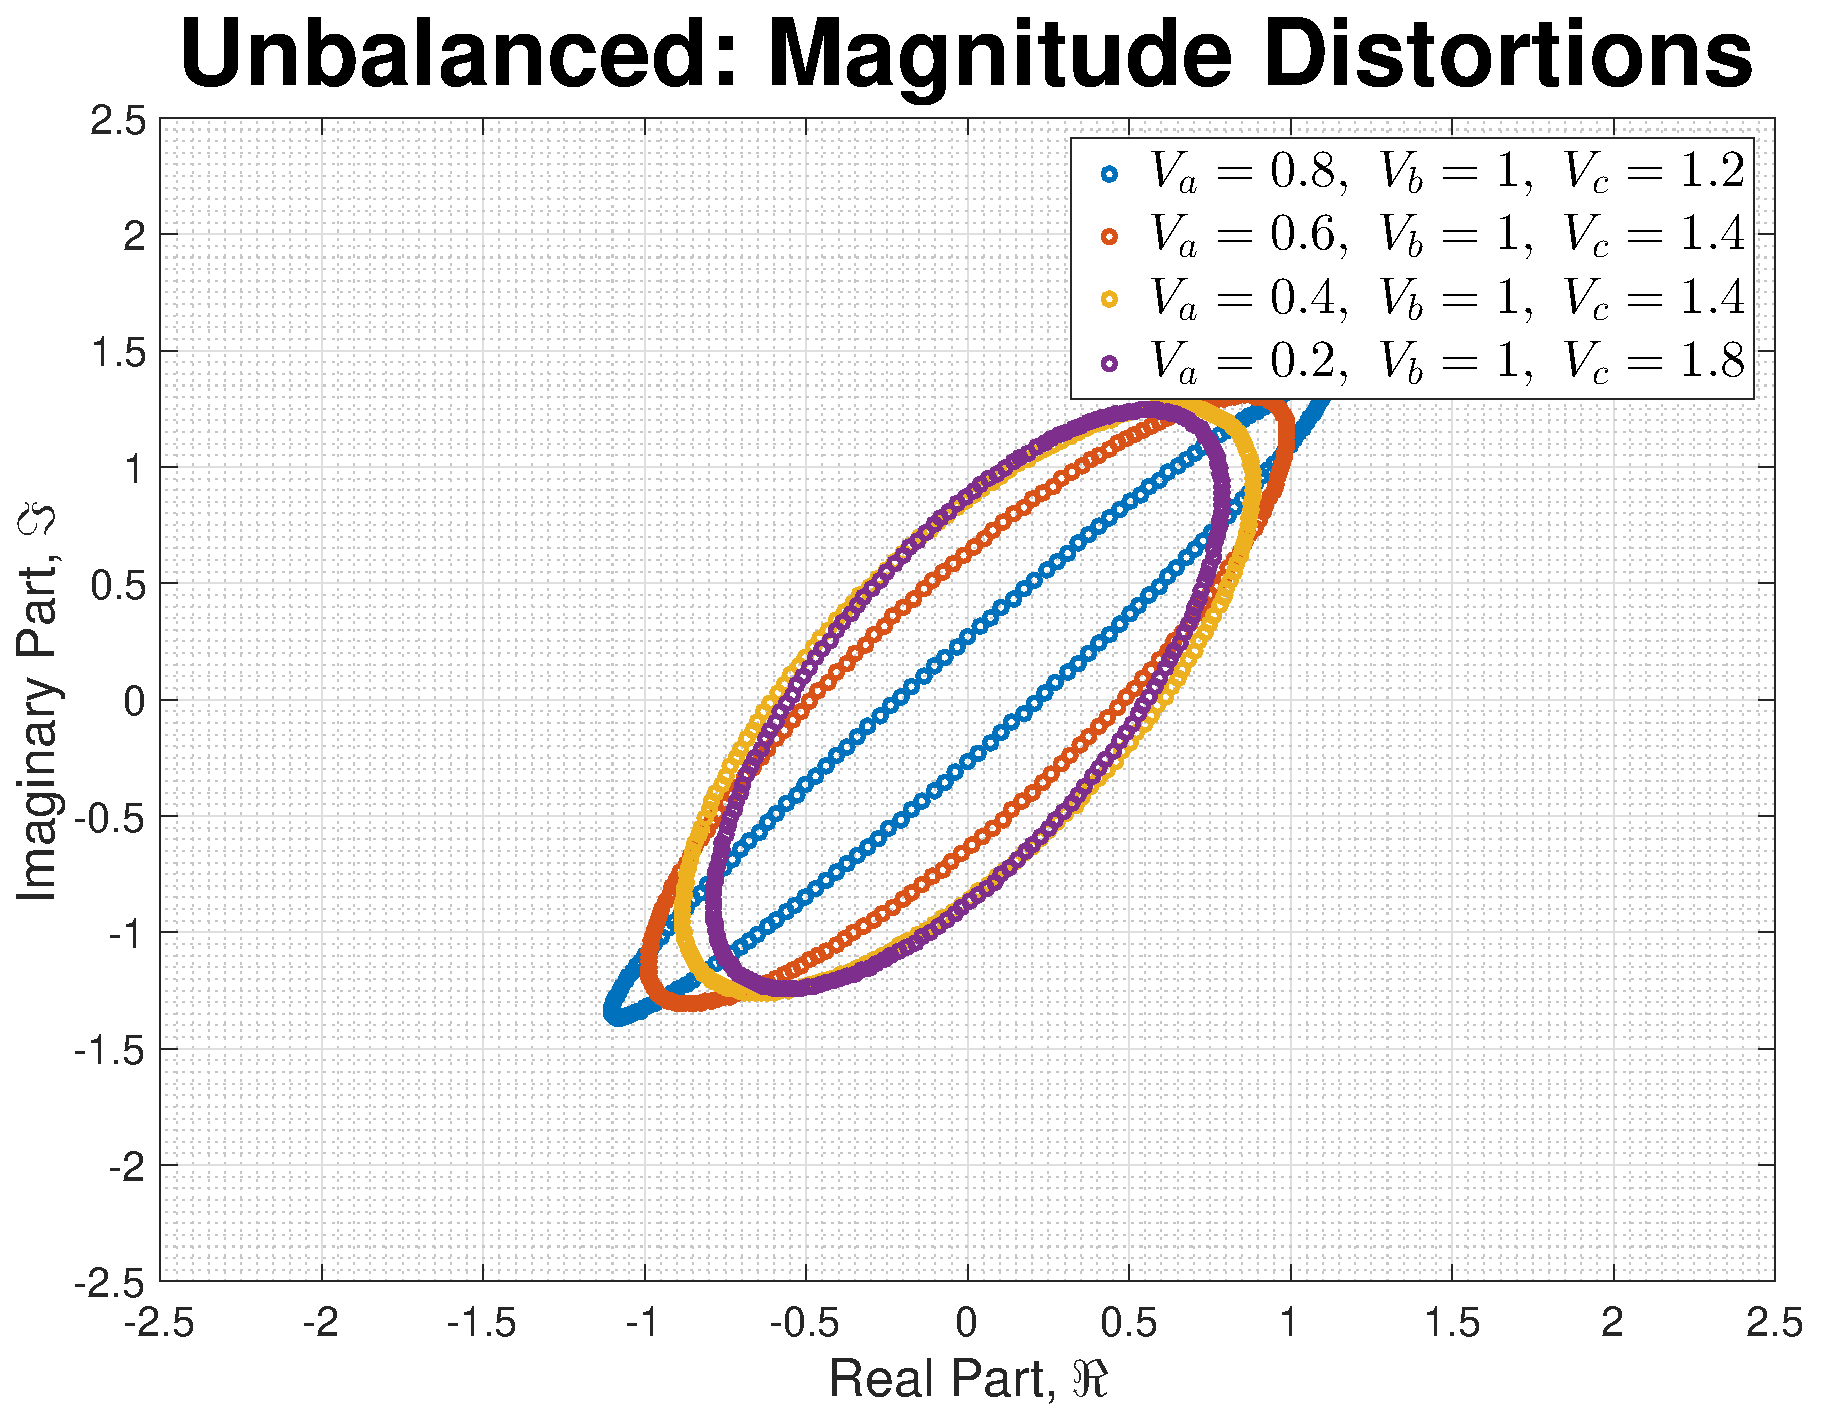
\includegraphics[width=0.32\textwidth]{part4/unbalanced_magnitude_distortion}
\caption{Balanced and Unbalanced Complex Voltages}
\end{figure}

\begin{figure}[H]
\centering{}
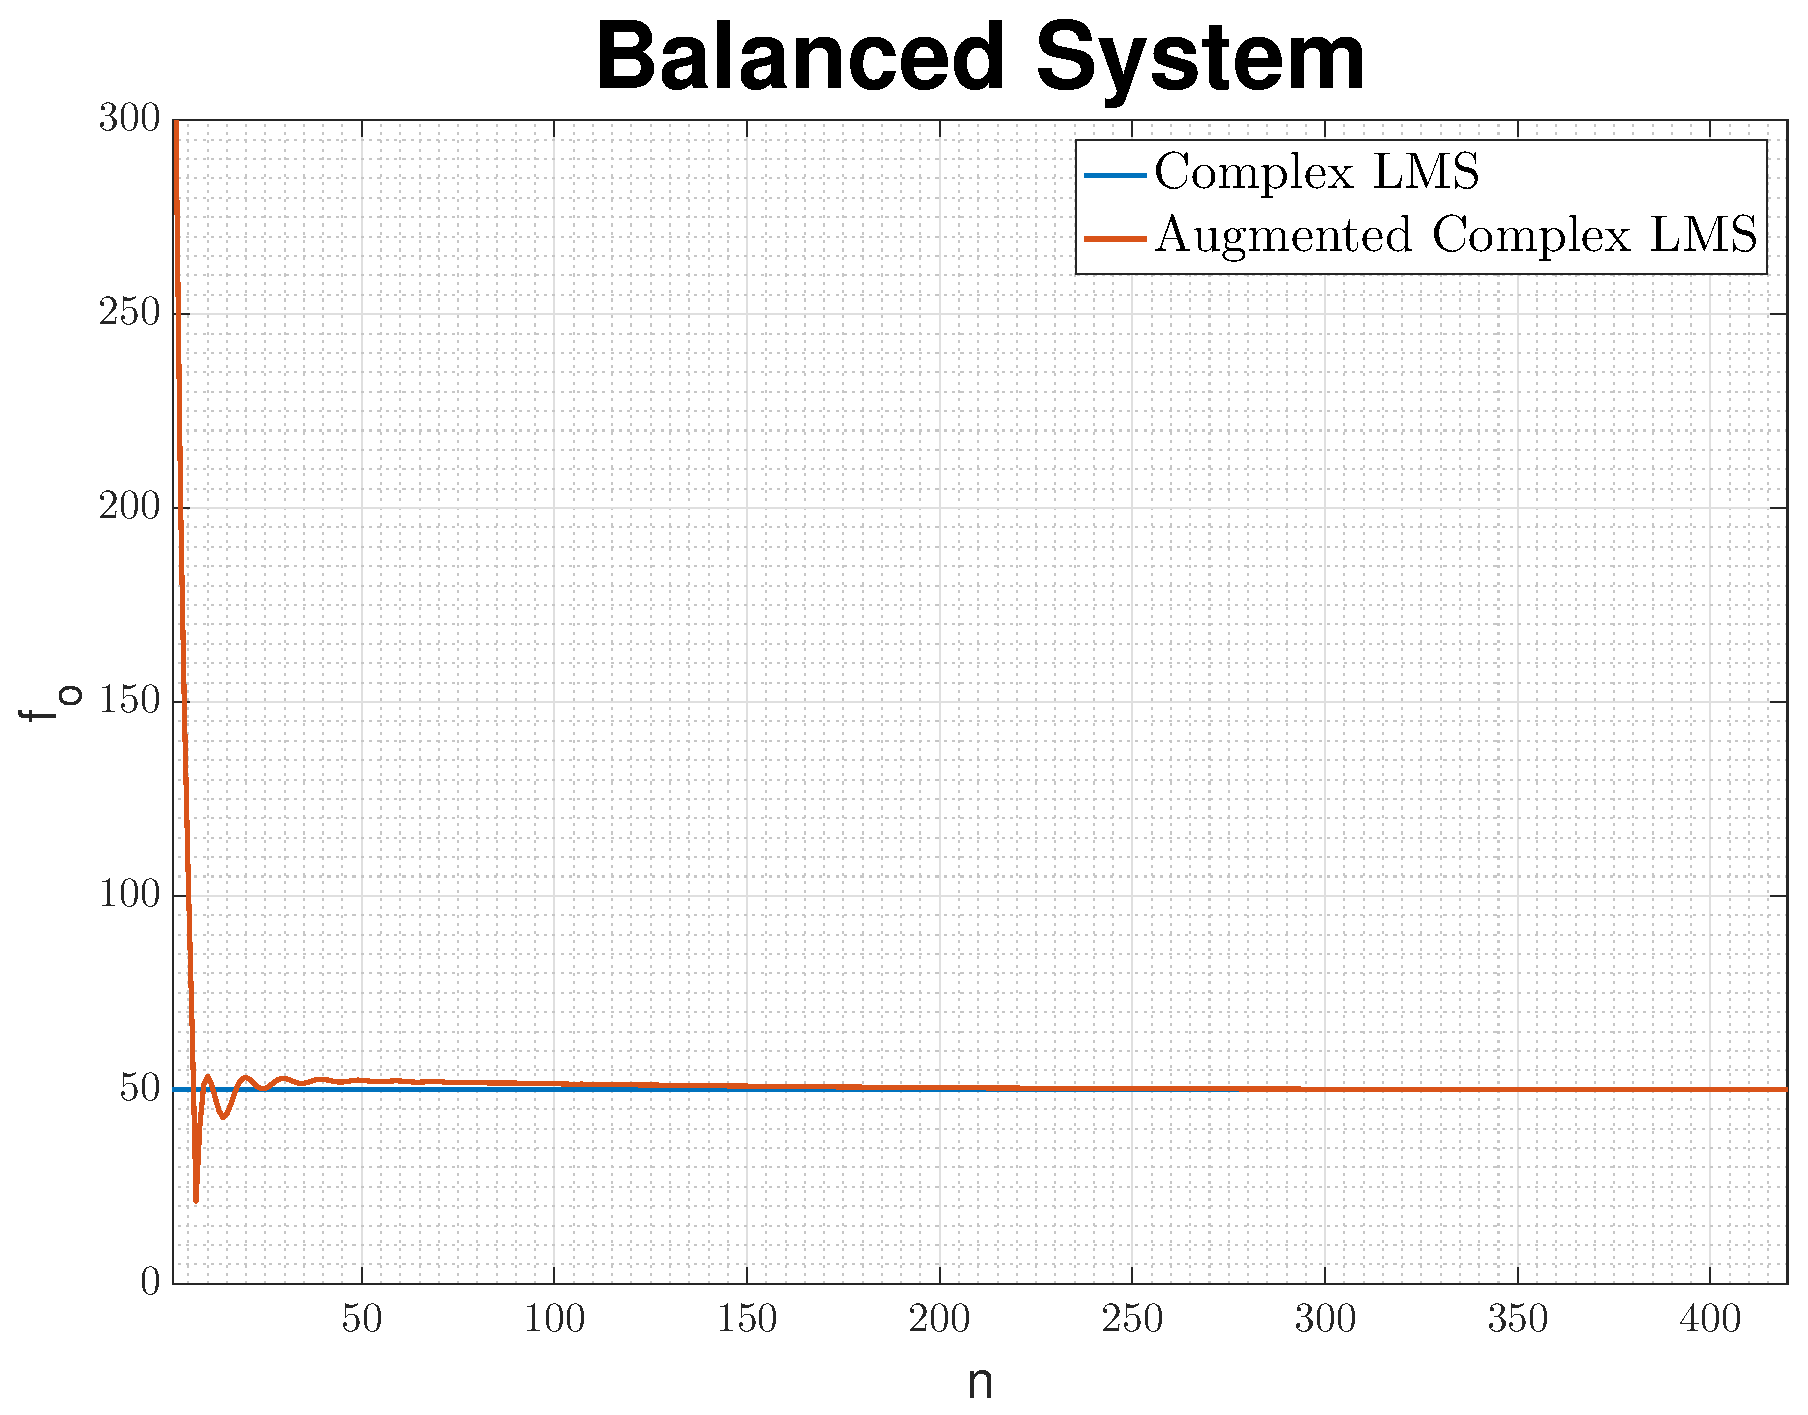
\includegraphics[width=0.32\textwidth]{part4/balanced_sys_clms_aclms}
\caption{Comparison of CLMS and ACLMS for Balanced Complex Voltages}
\end{figure}

\begin{figure}[H]
\centering{}
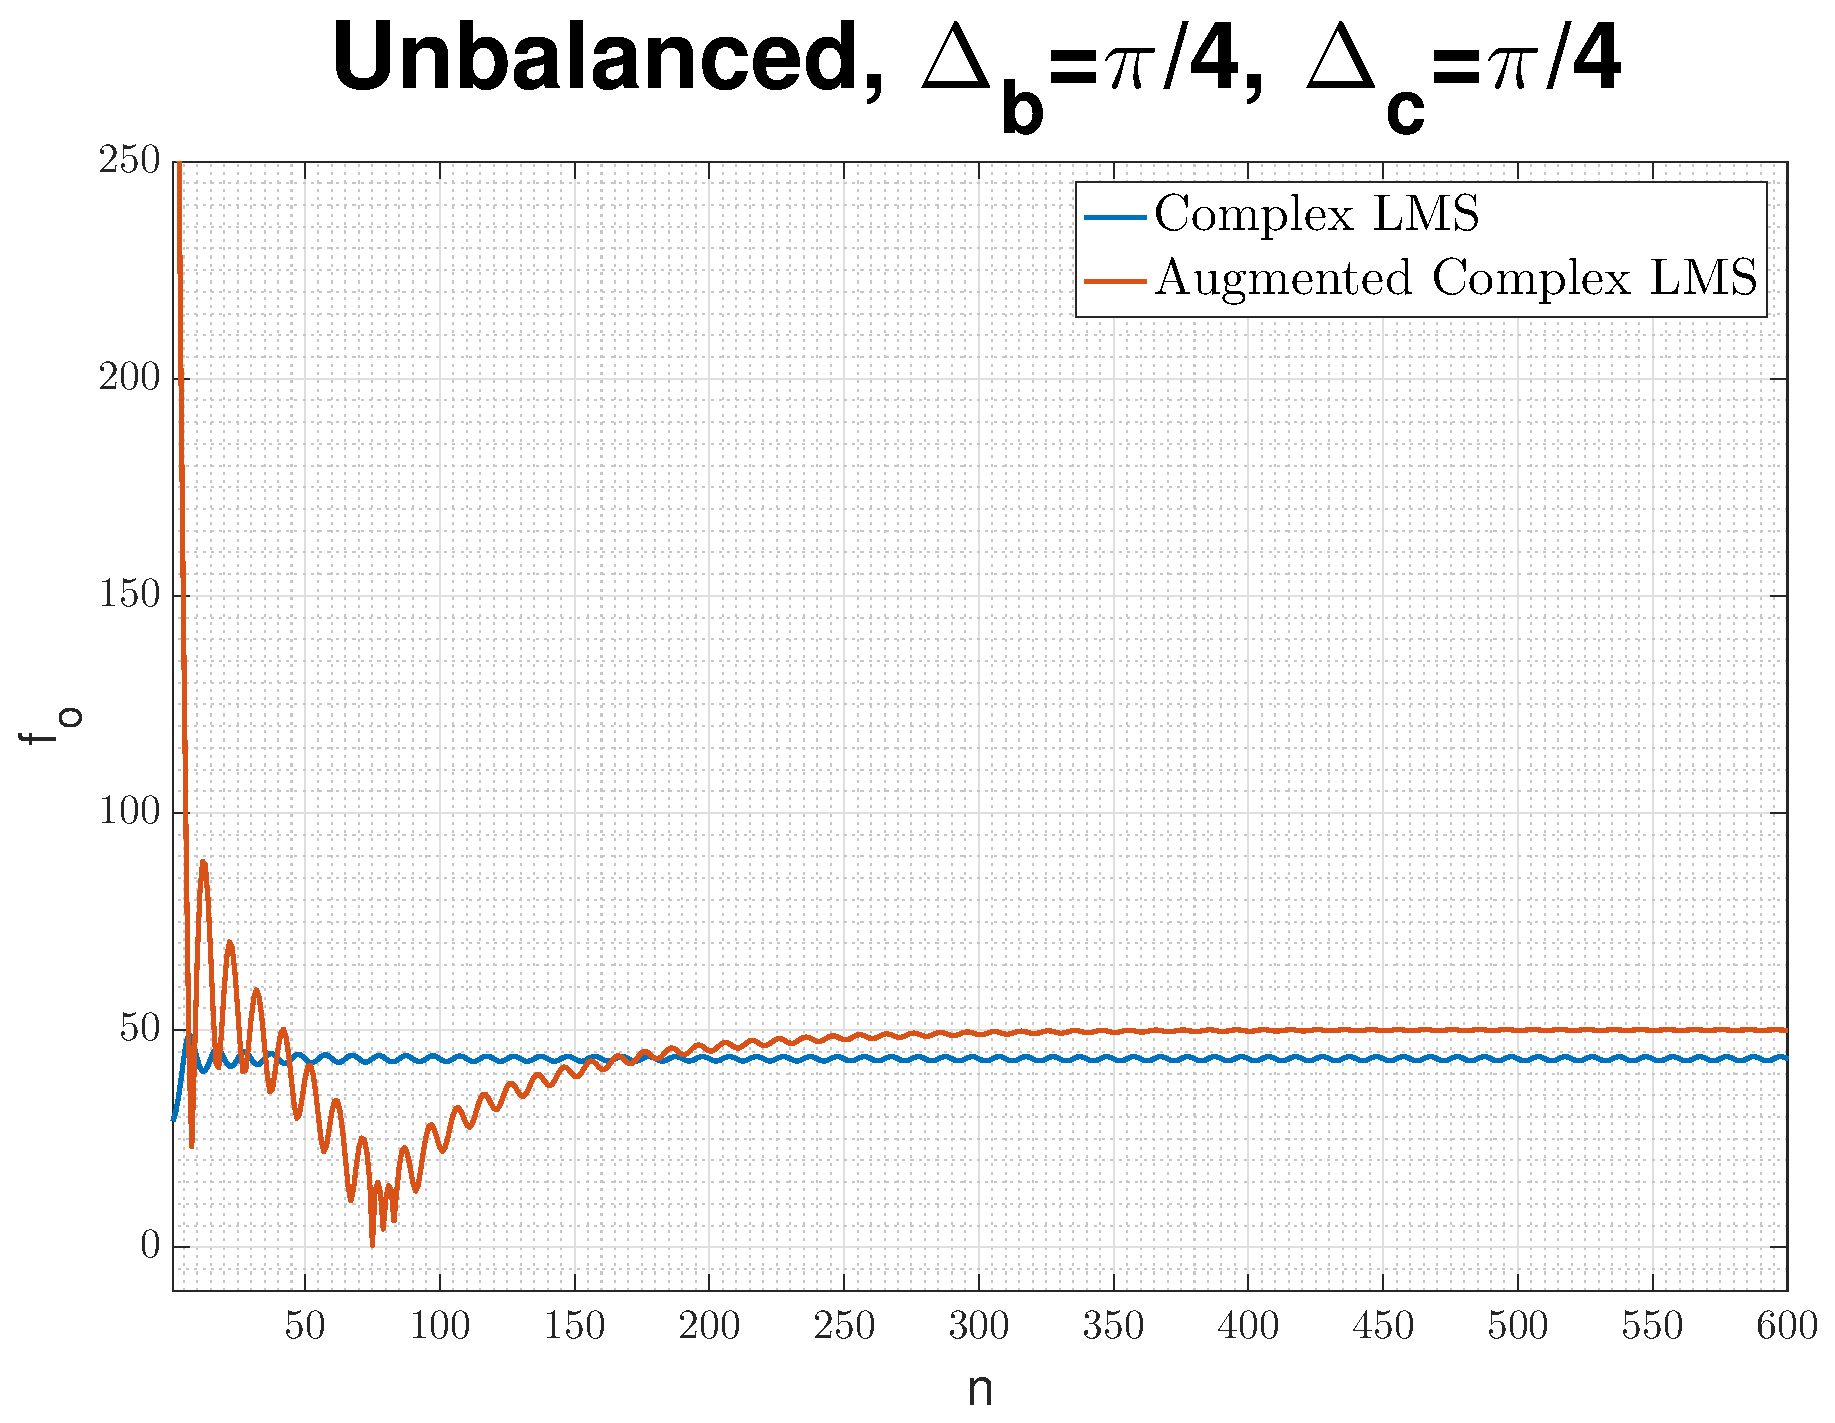
\includegraphics[width=0.32\textwidth]{part4/unbalanced_sys_clms_aclms_phase}
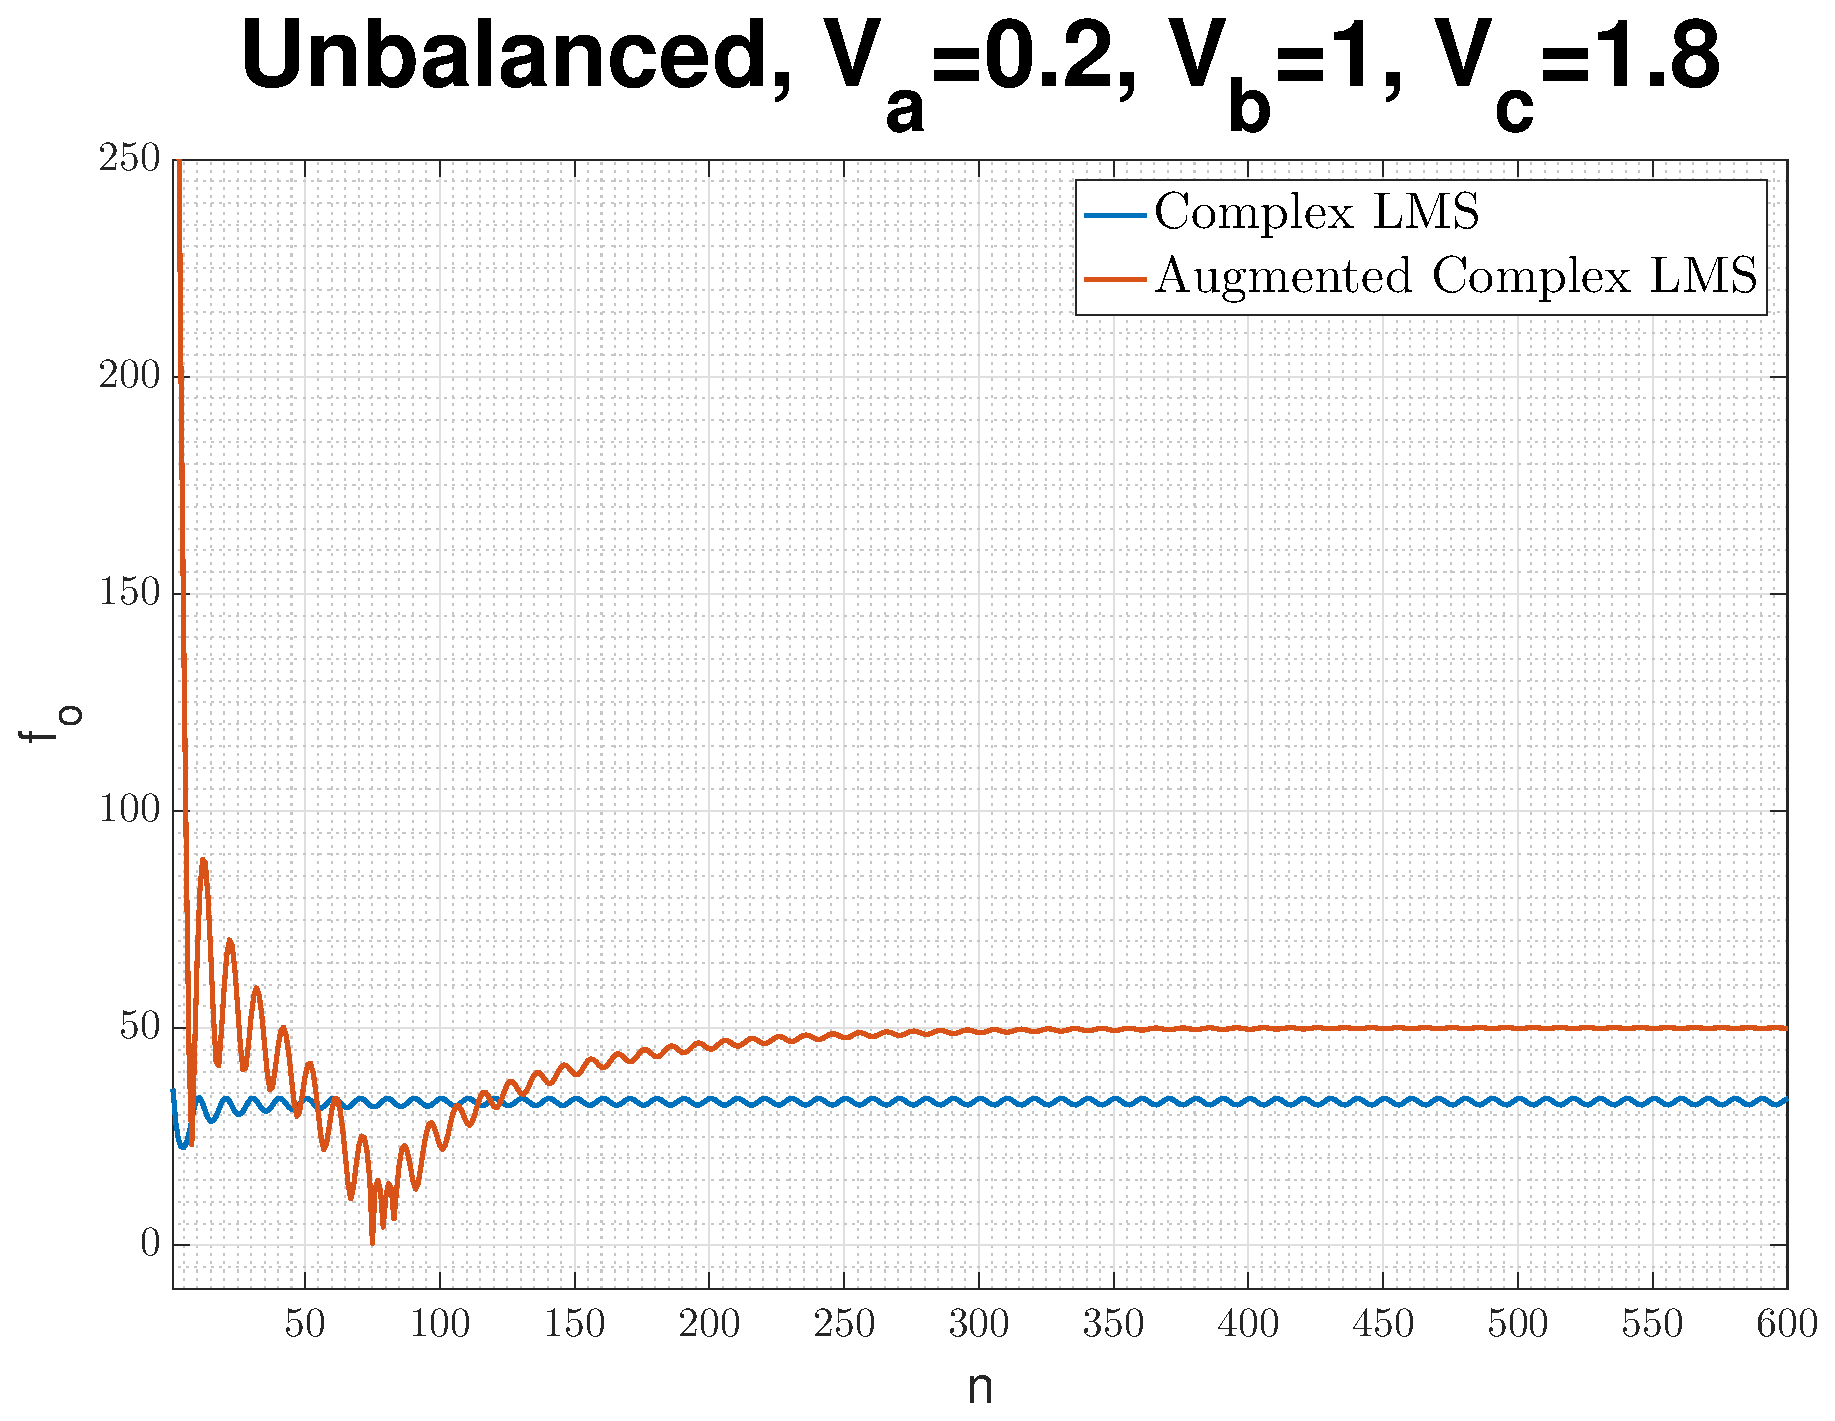
\includegraphics[width=0.32\textwidth]{part4/unbalanced_sys_clms_aclms_magnitude}
\caption{Comparison of CLMS and ACLMS for Unbalanced Complex Voltages}
\end{figure}

\begin{figure}[H]
\centering{}
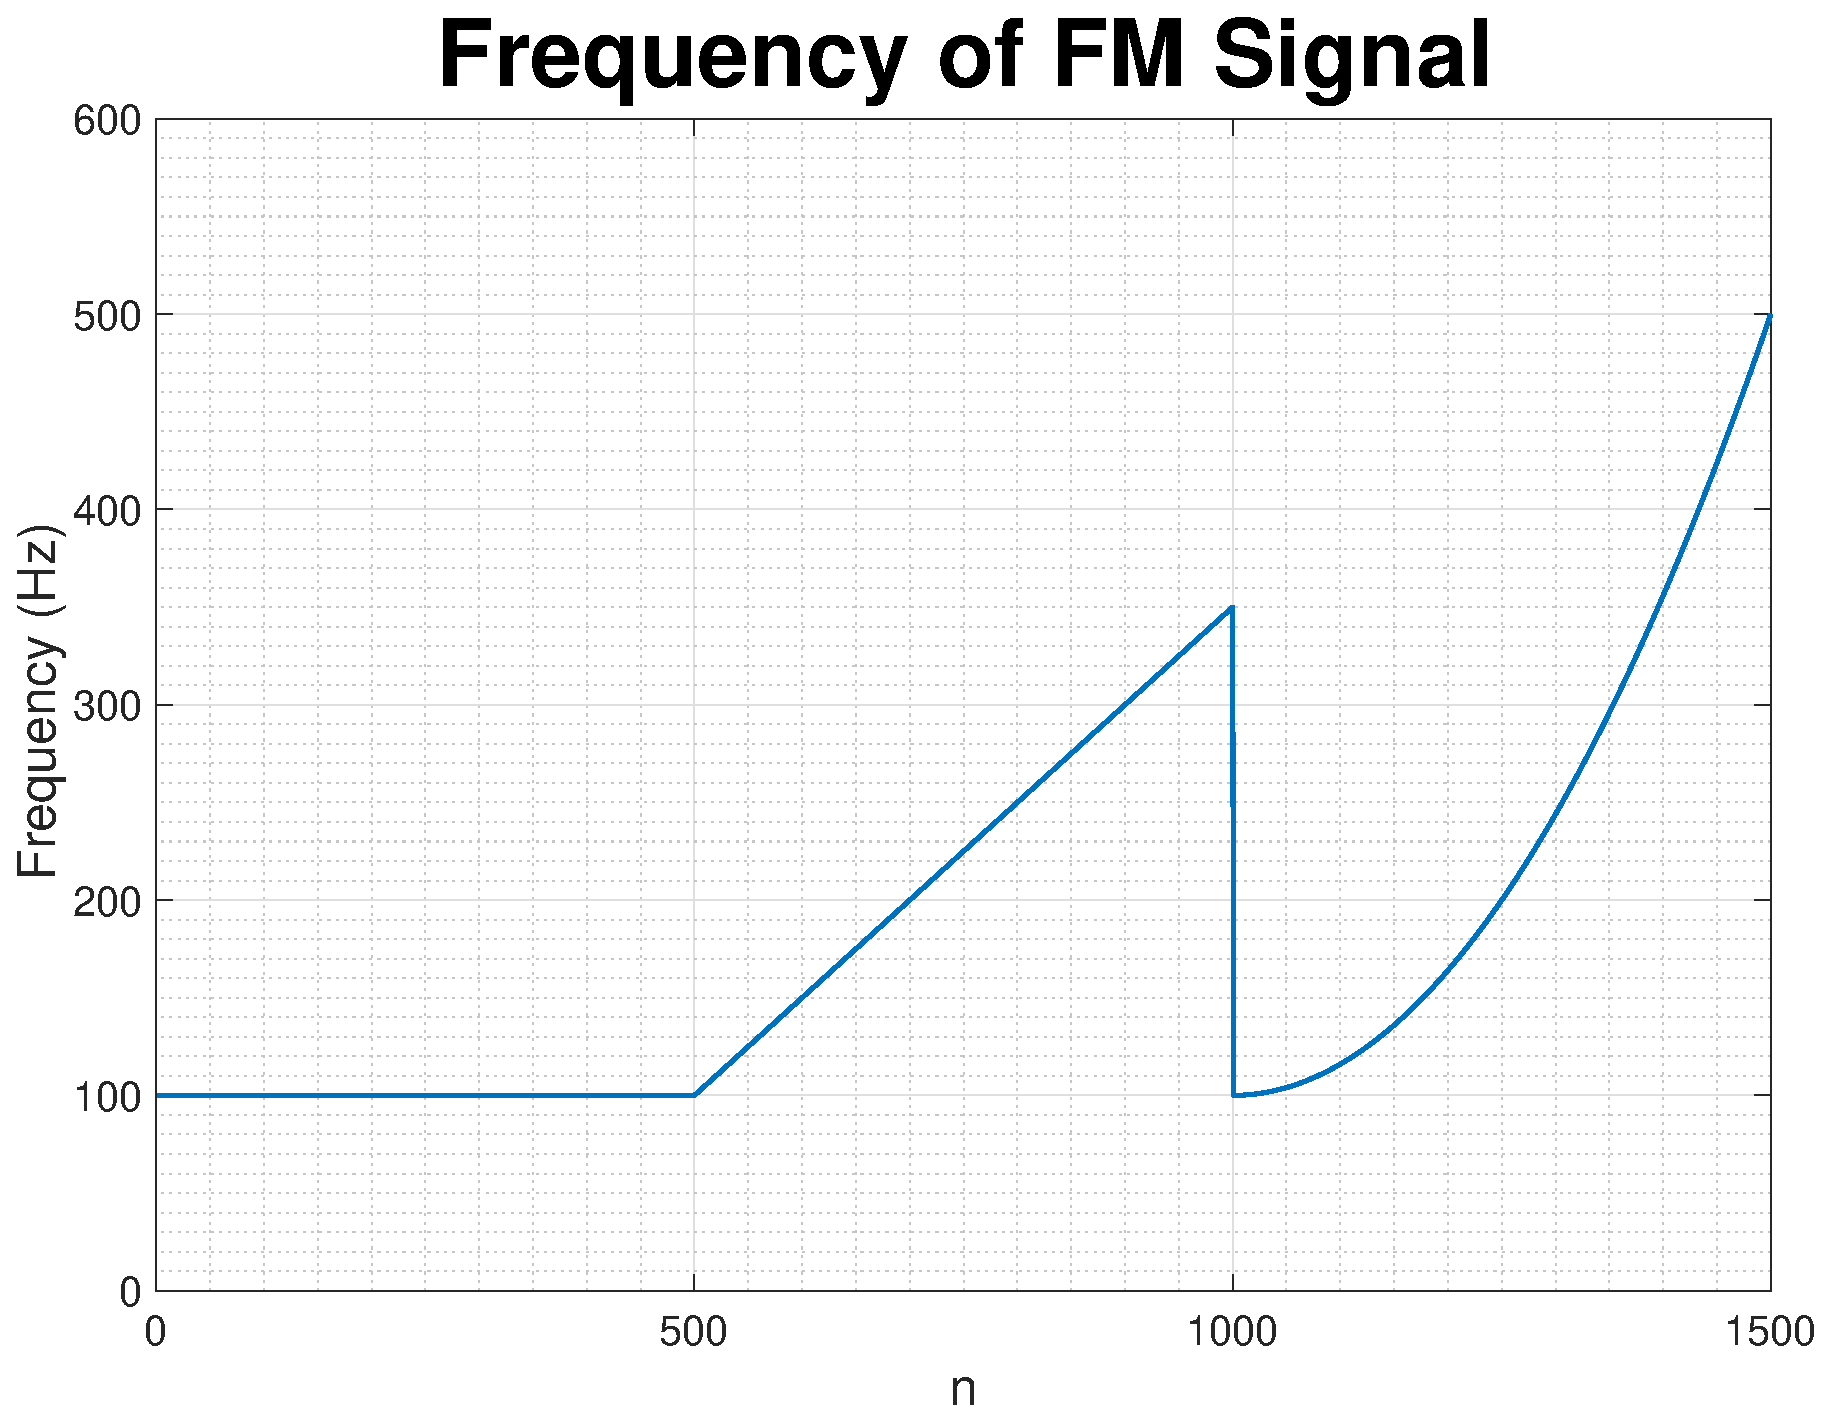
\includegraphics[width=0.32\textwidth]{part4/frequency_original_fm_signal}
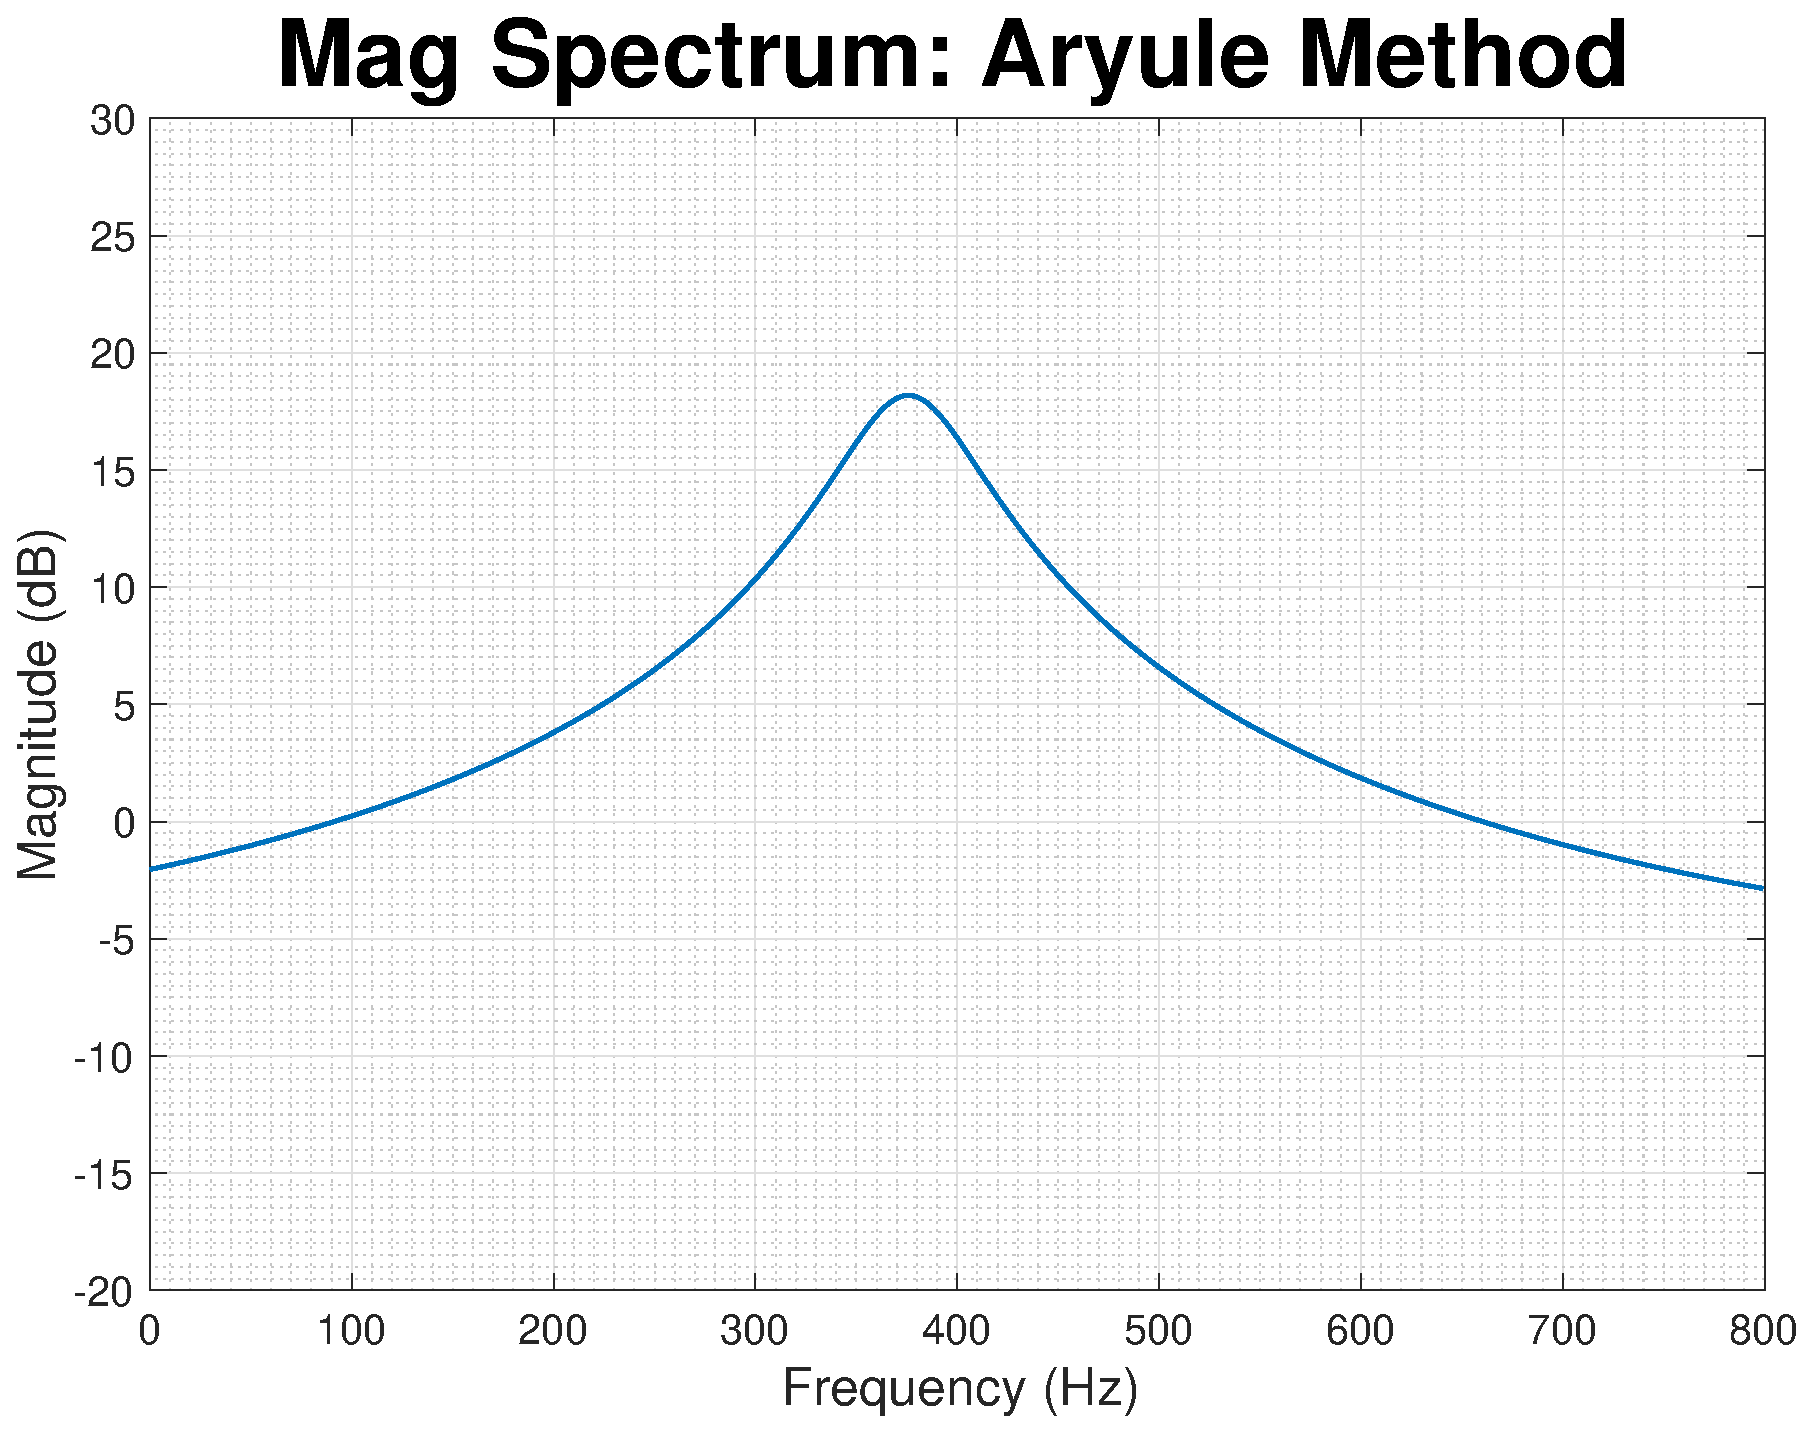
\includegraphics[width=0.32\textwidth]{part4/frequency_aryule_fm_signal}
\caption{Original, Non-Stationary Frequency of FM Signal and Power Spectrum obtained using Block-Based Estimate of AR Coefficients}
\end{figure}

\begin{figure}[H]
\centering{}
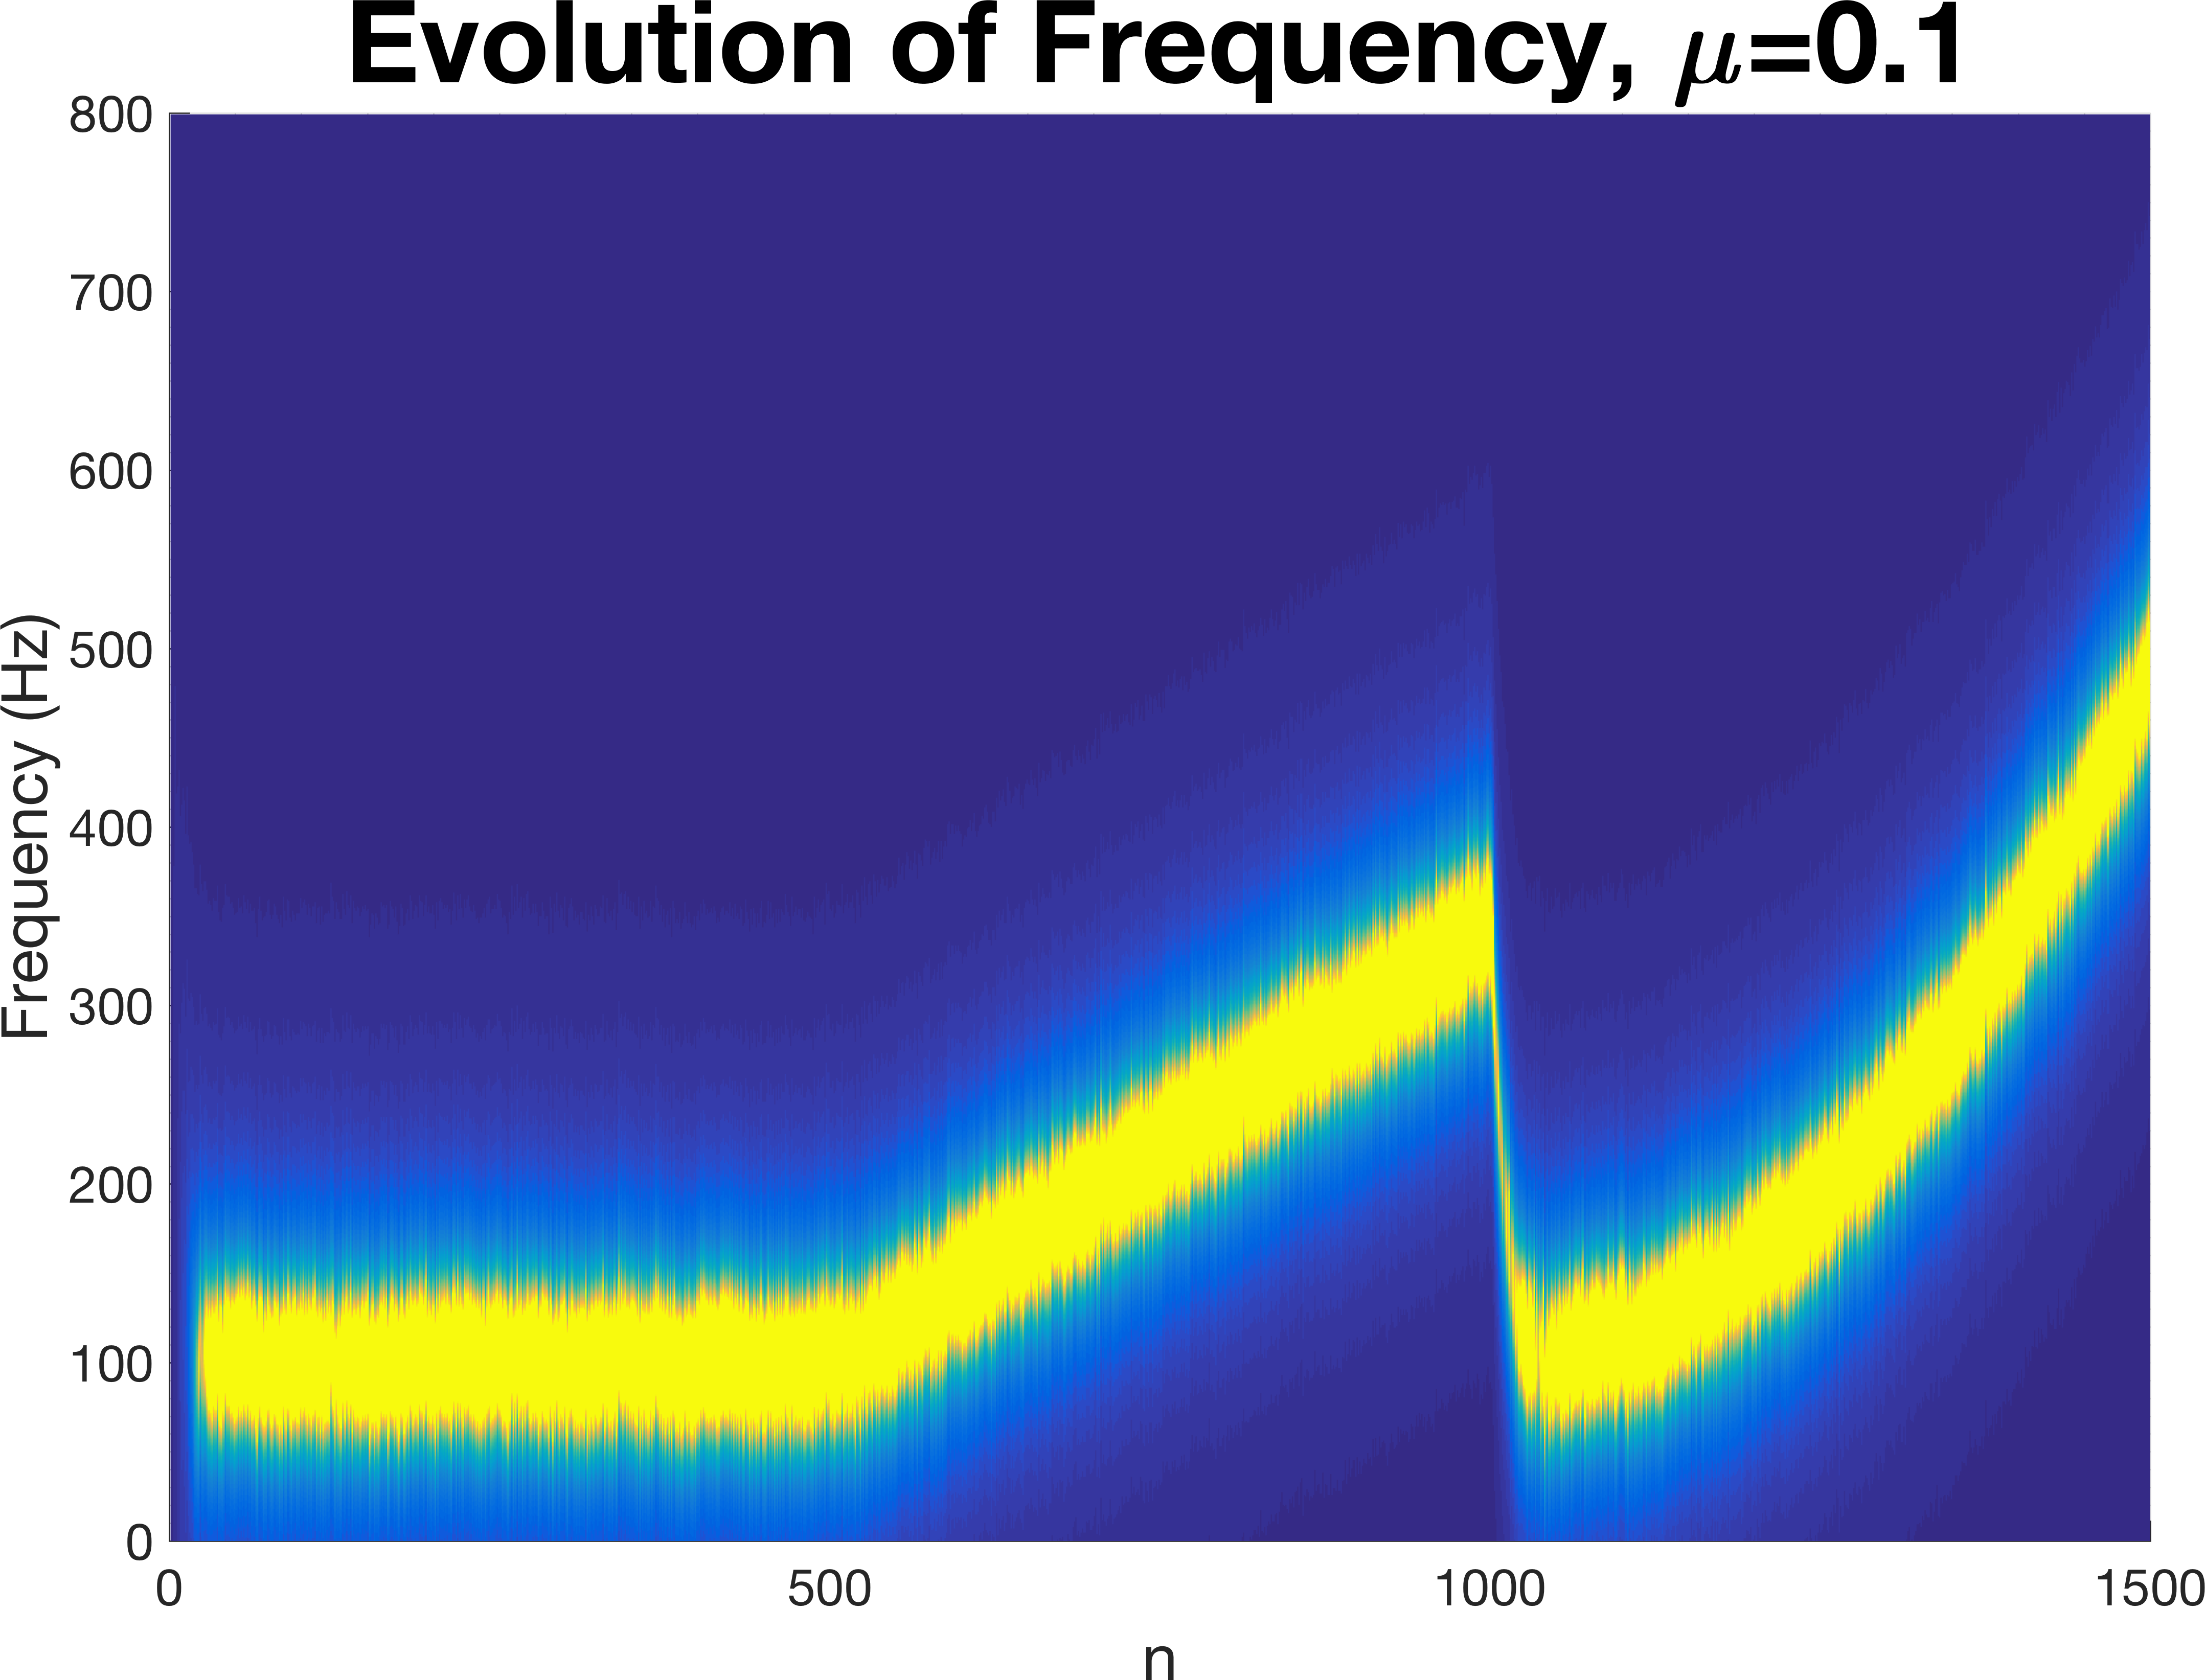
\includegraphics[width=0.32\textwidth]{part4/frequency_clms_fm_signal_1}
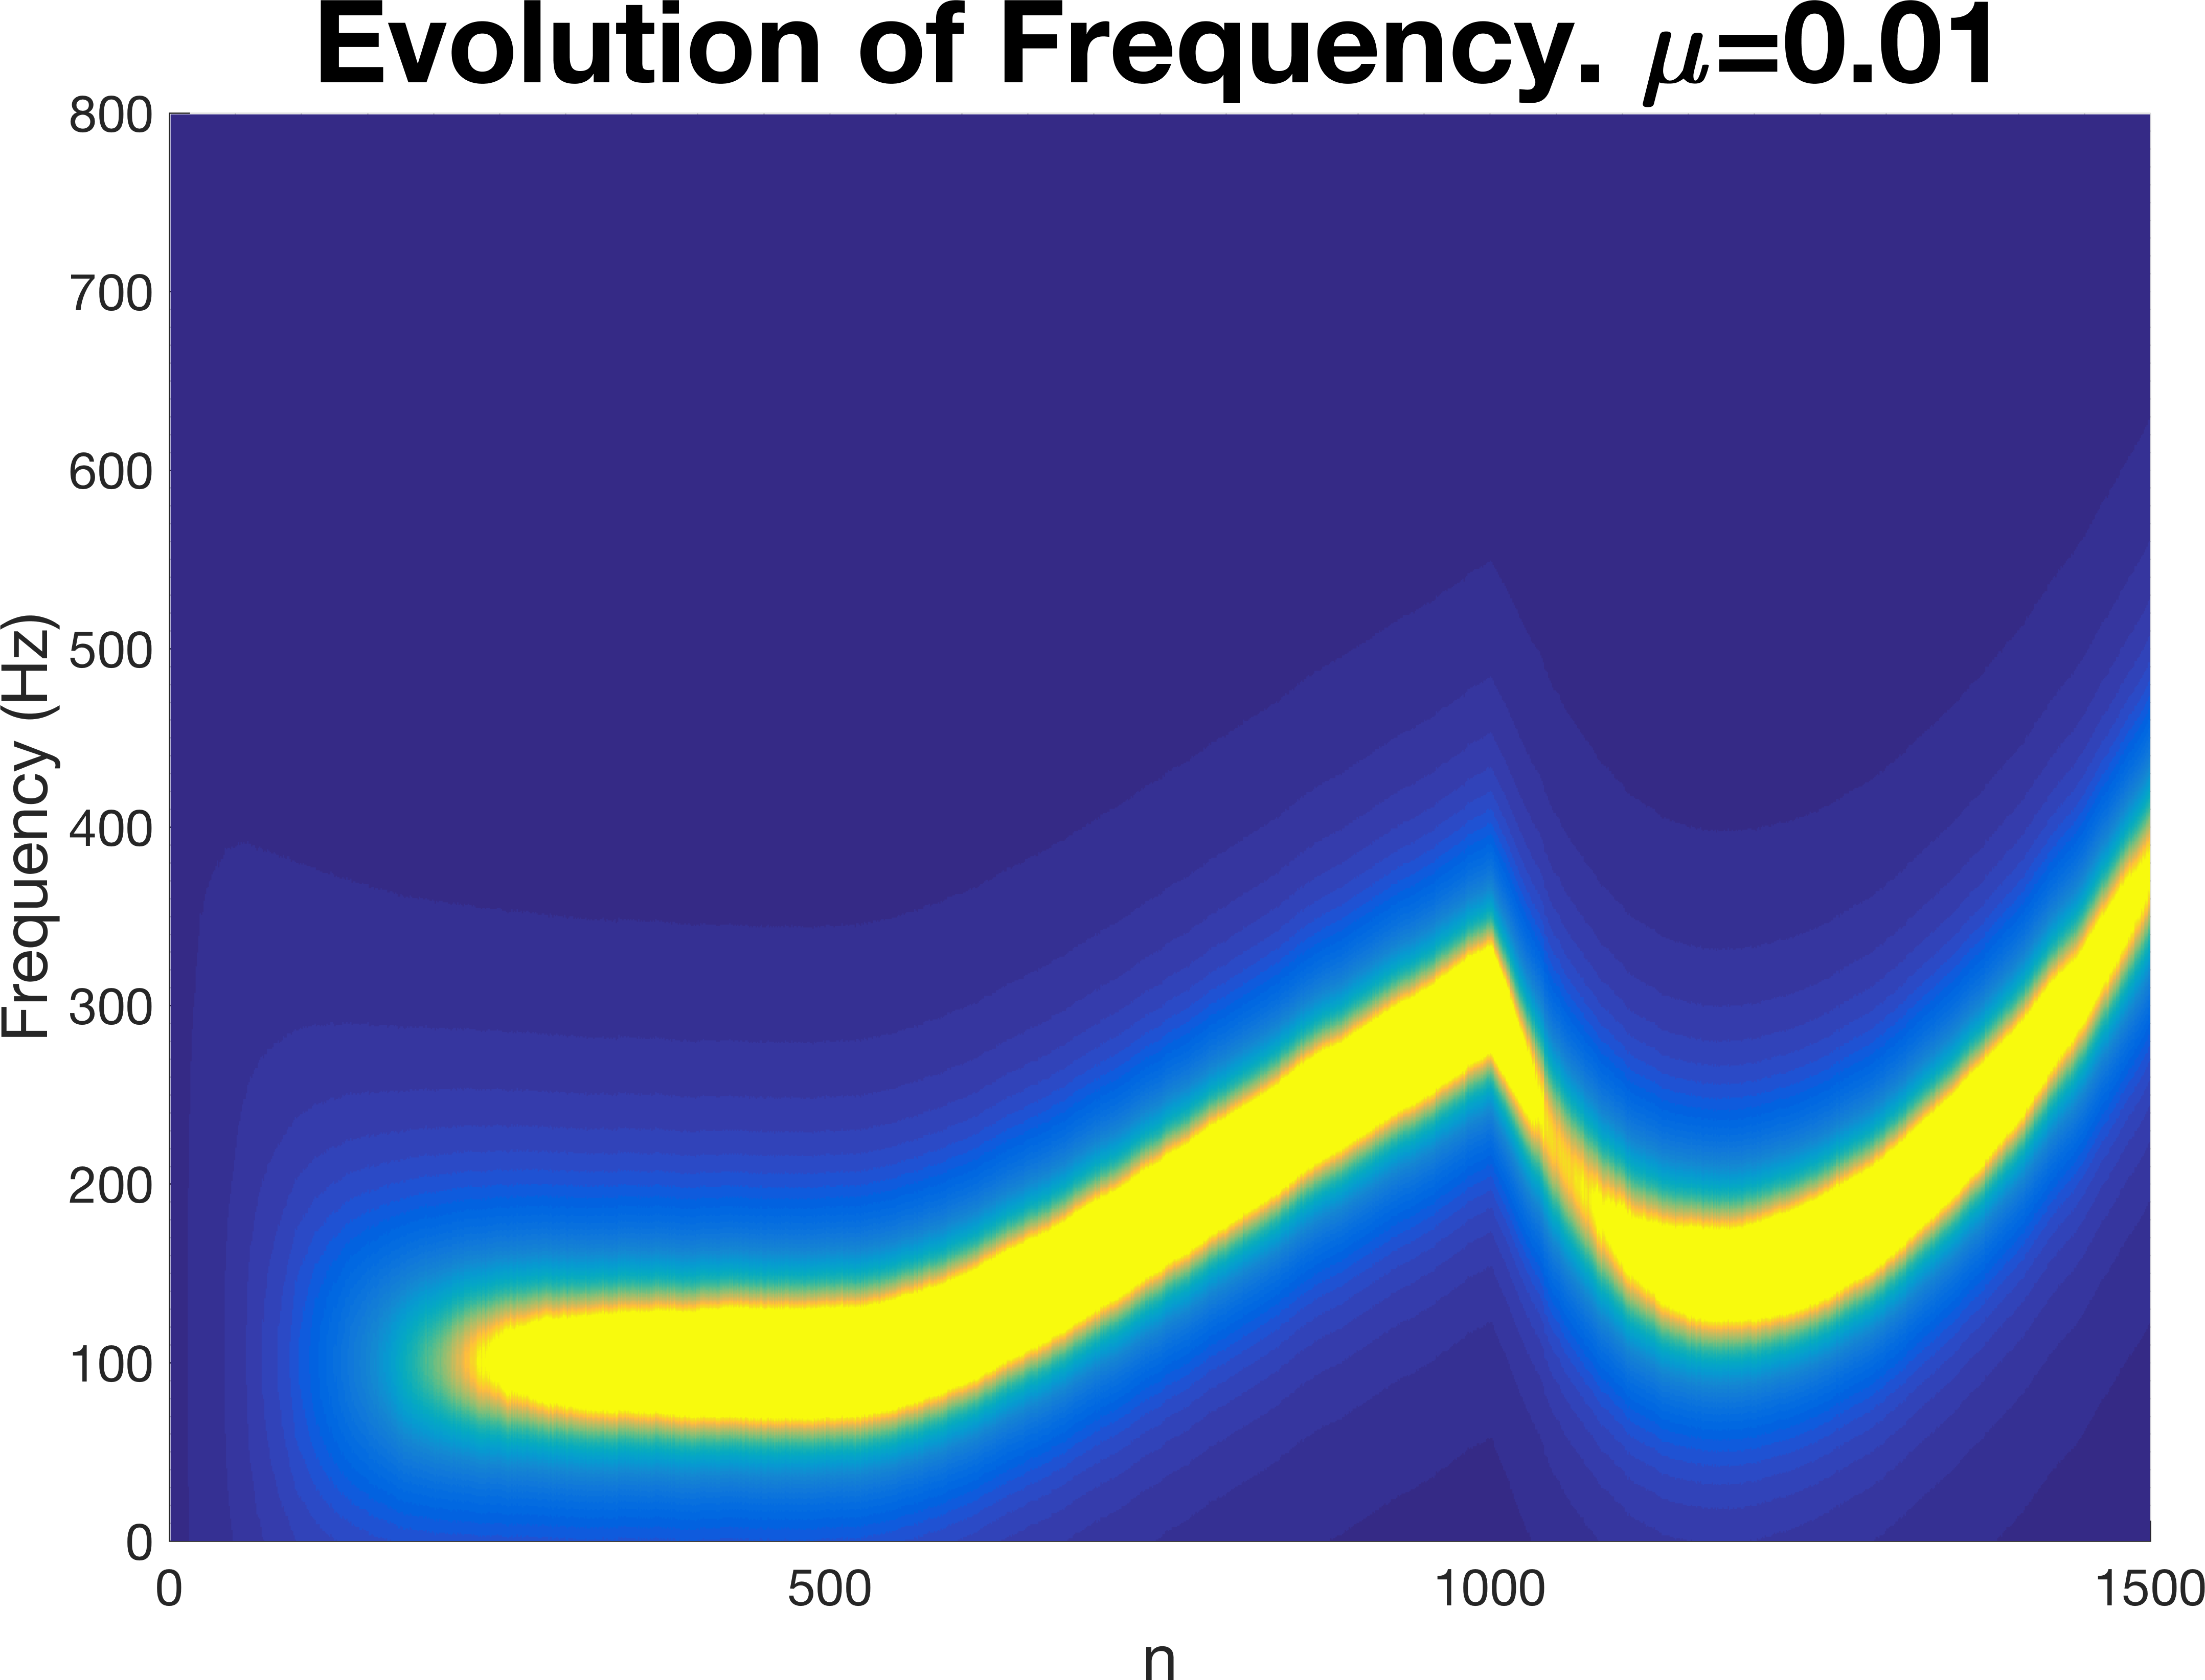
\includegraphics[width=0.32\textwidth]{part4/frequency_clms_fm_signal_01}
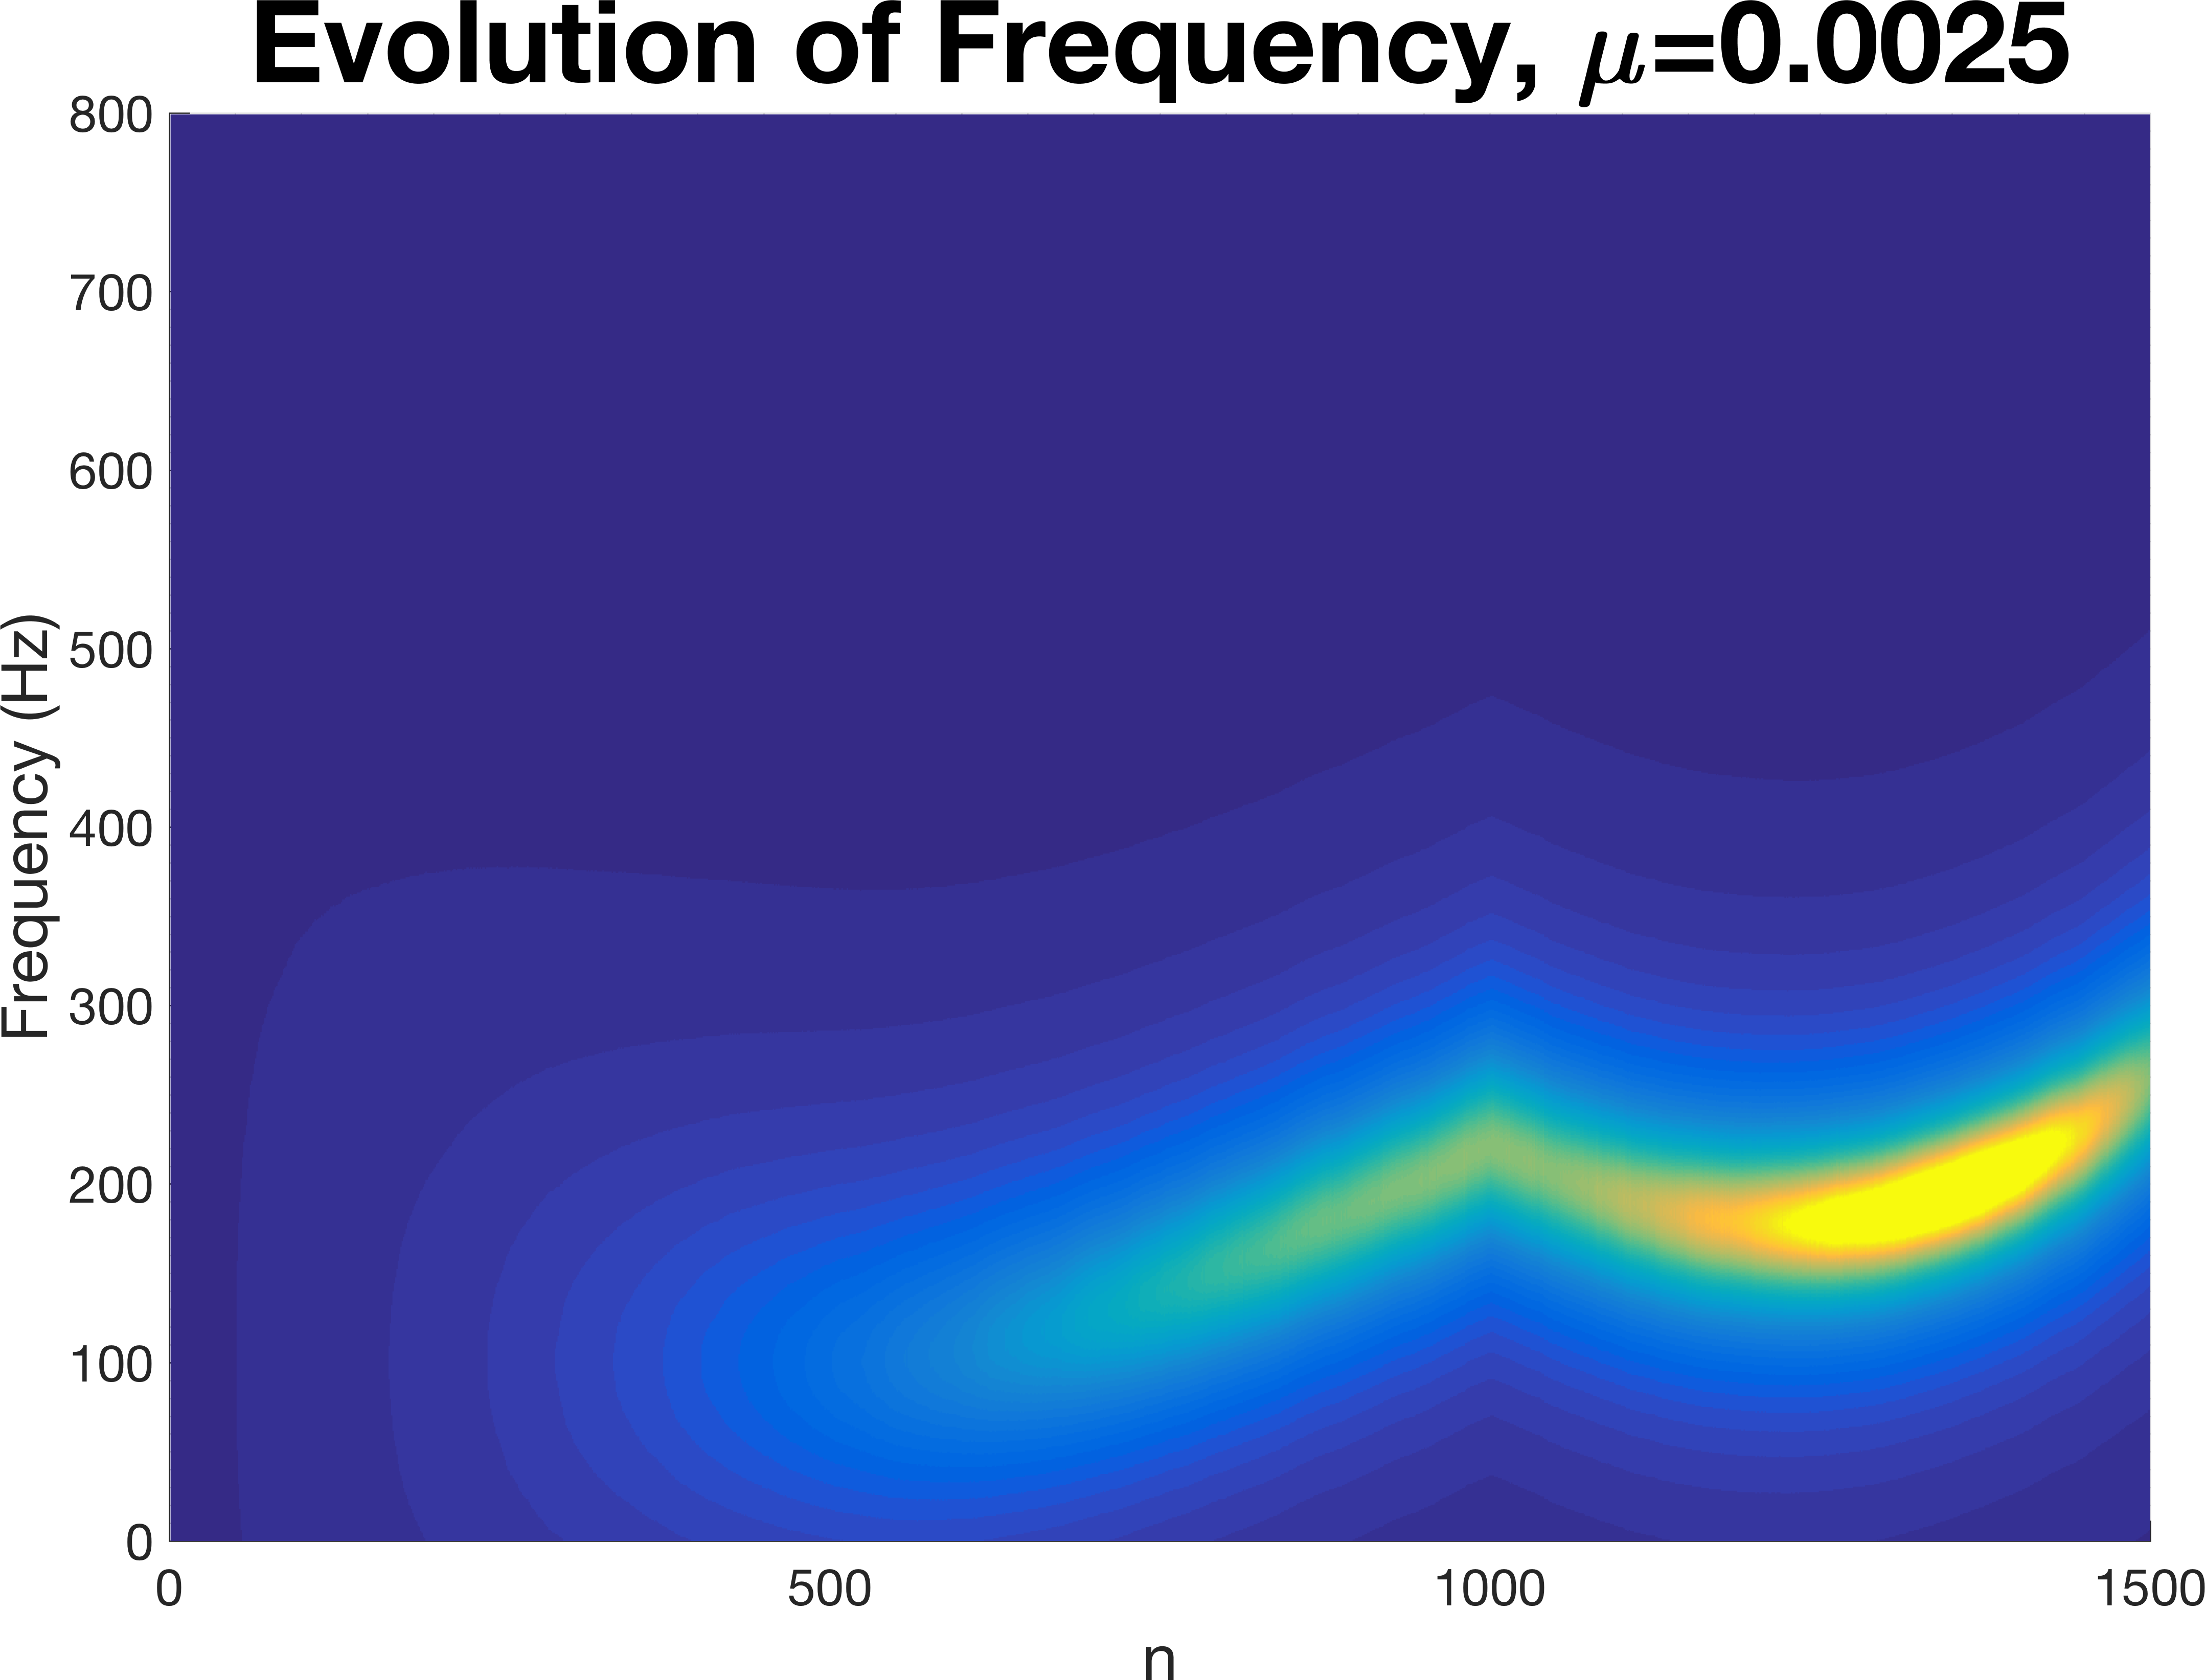
\includegraphics[width=0.32\textwidth]{part4/frequency_clms_fm_signal_0025}
\caption{Time-Frequency Estimation using Complex LMS Algorithm with Different Values of $\mu$}
\end{figure}

\begin{figure}[H]
\centering{}
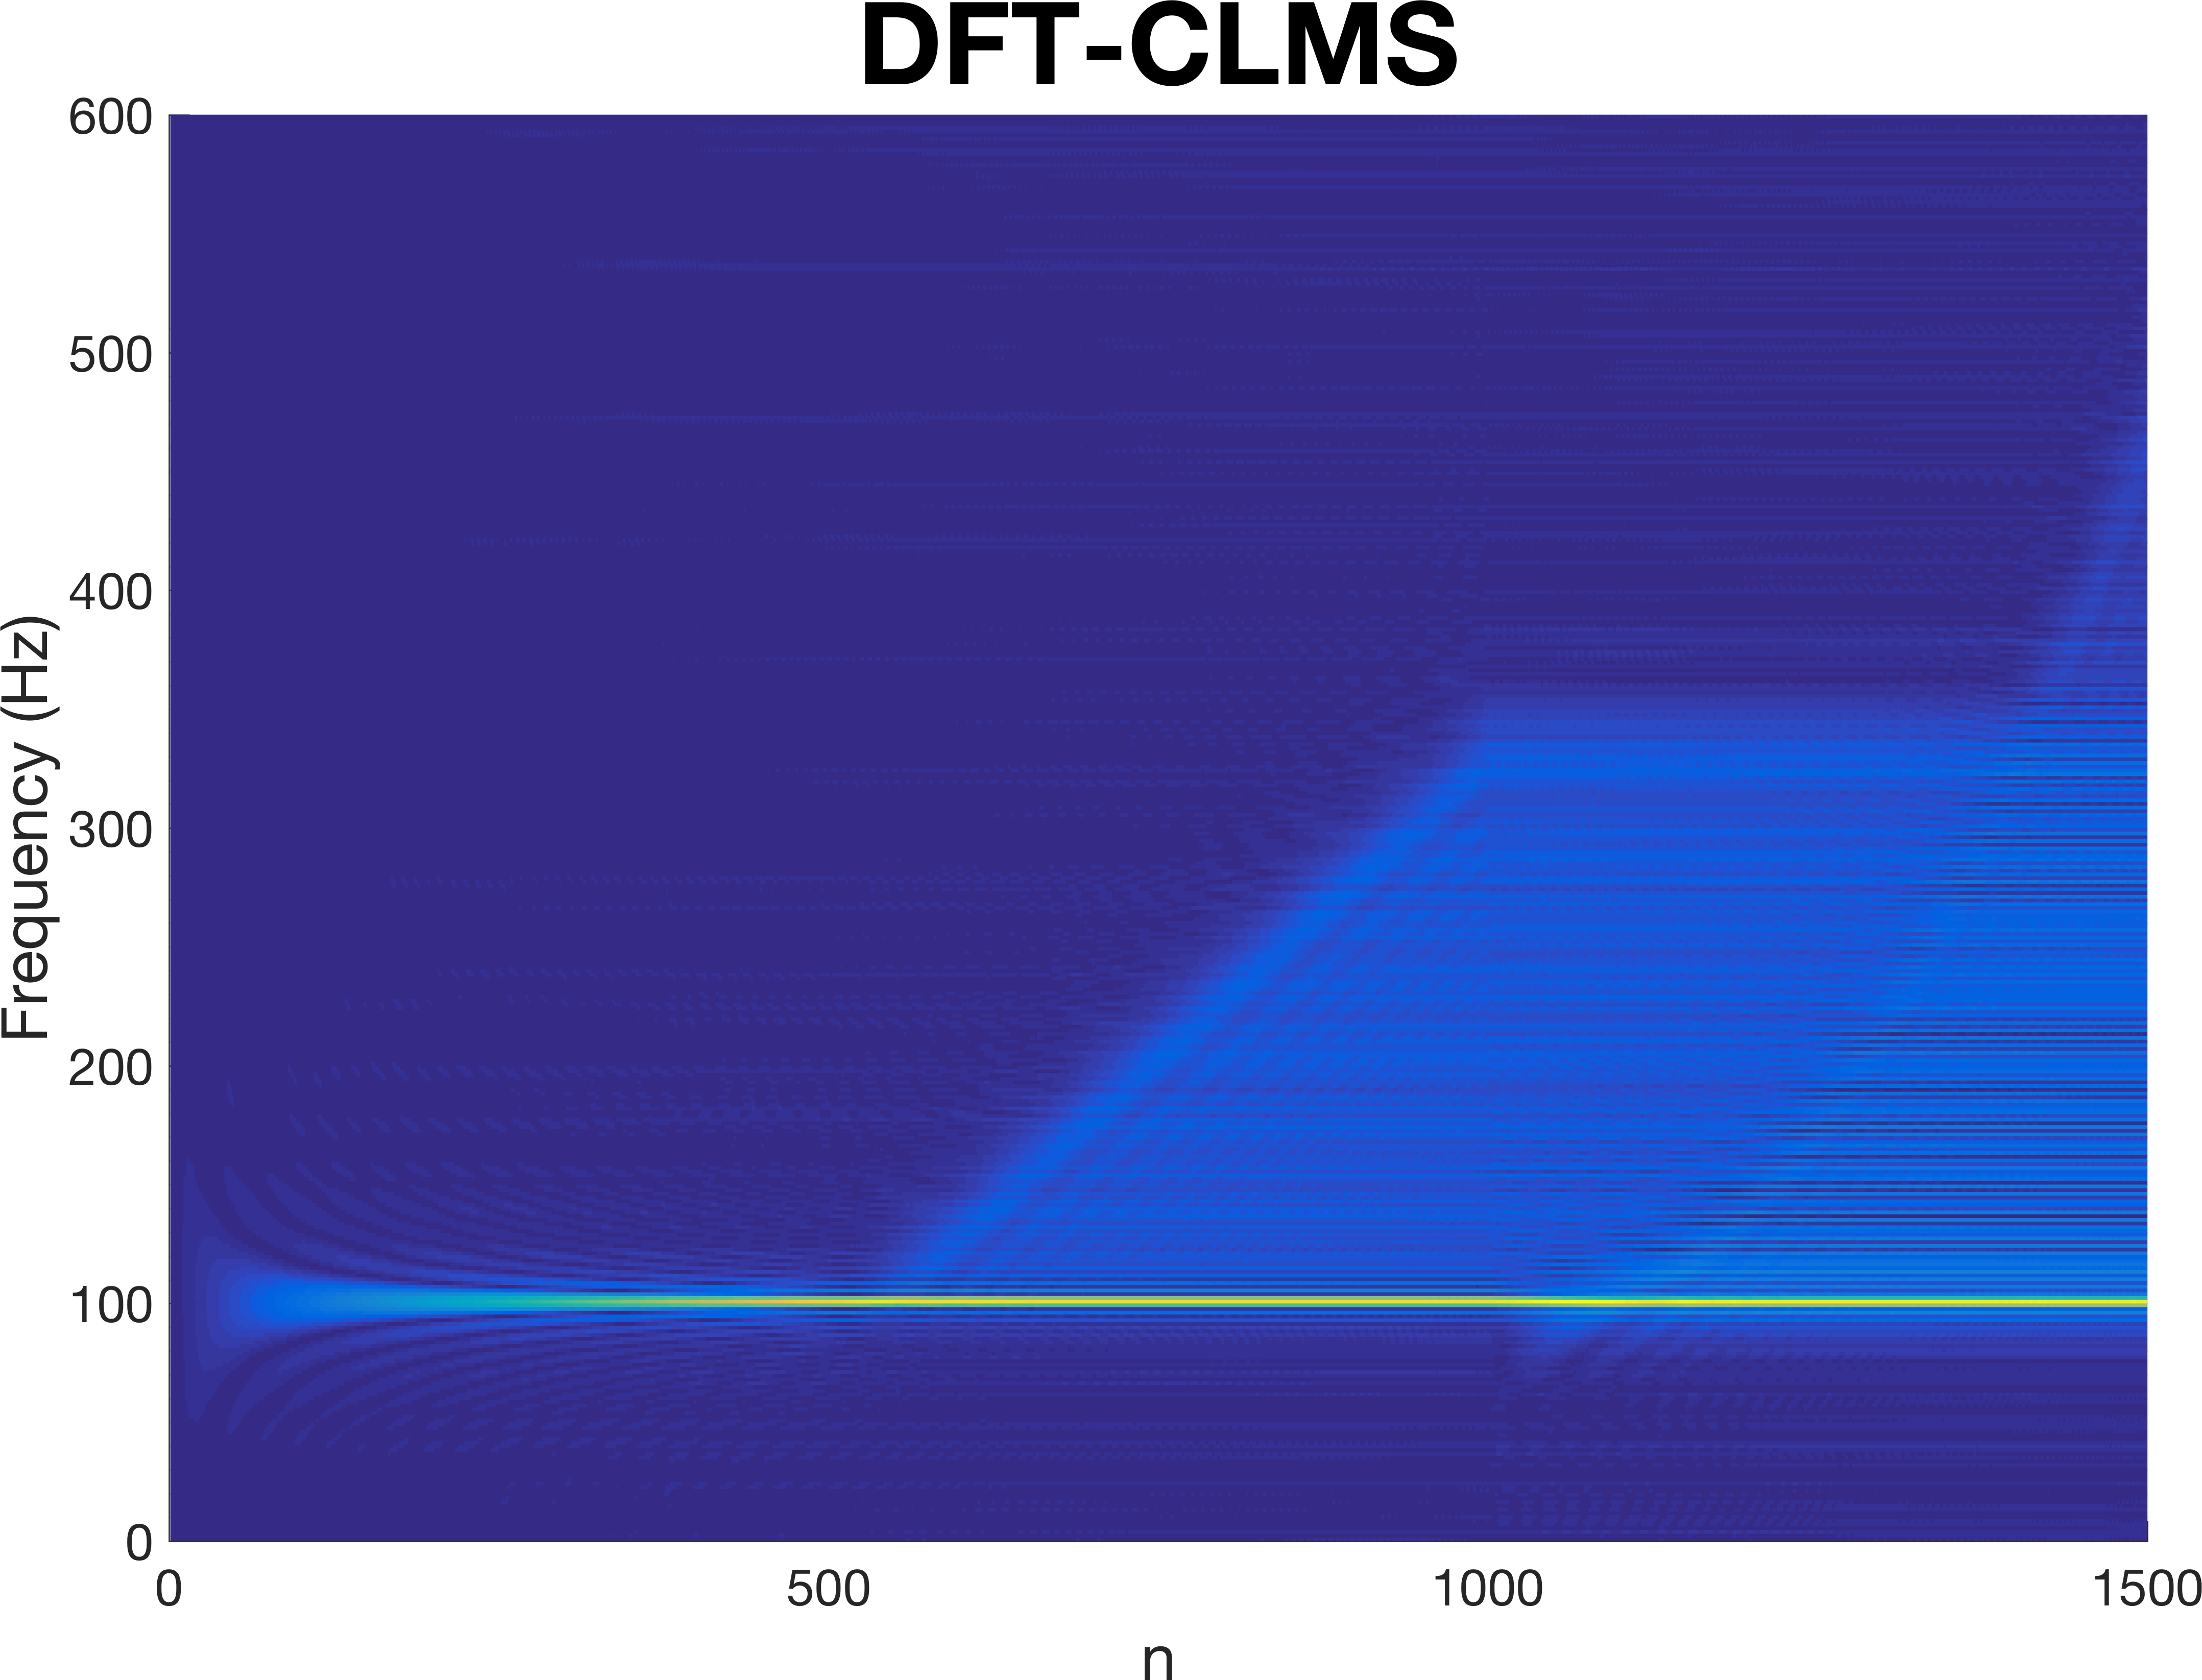
\includegraphics[width=0.32\textwidth]{part4/time_frequency_dft_non_leaky}
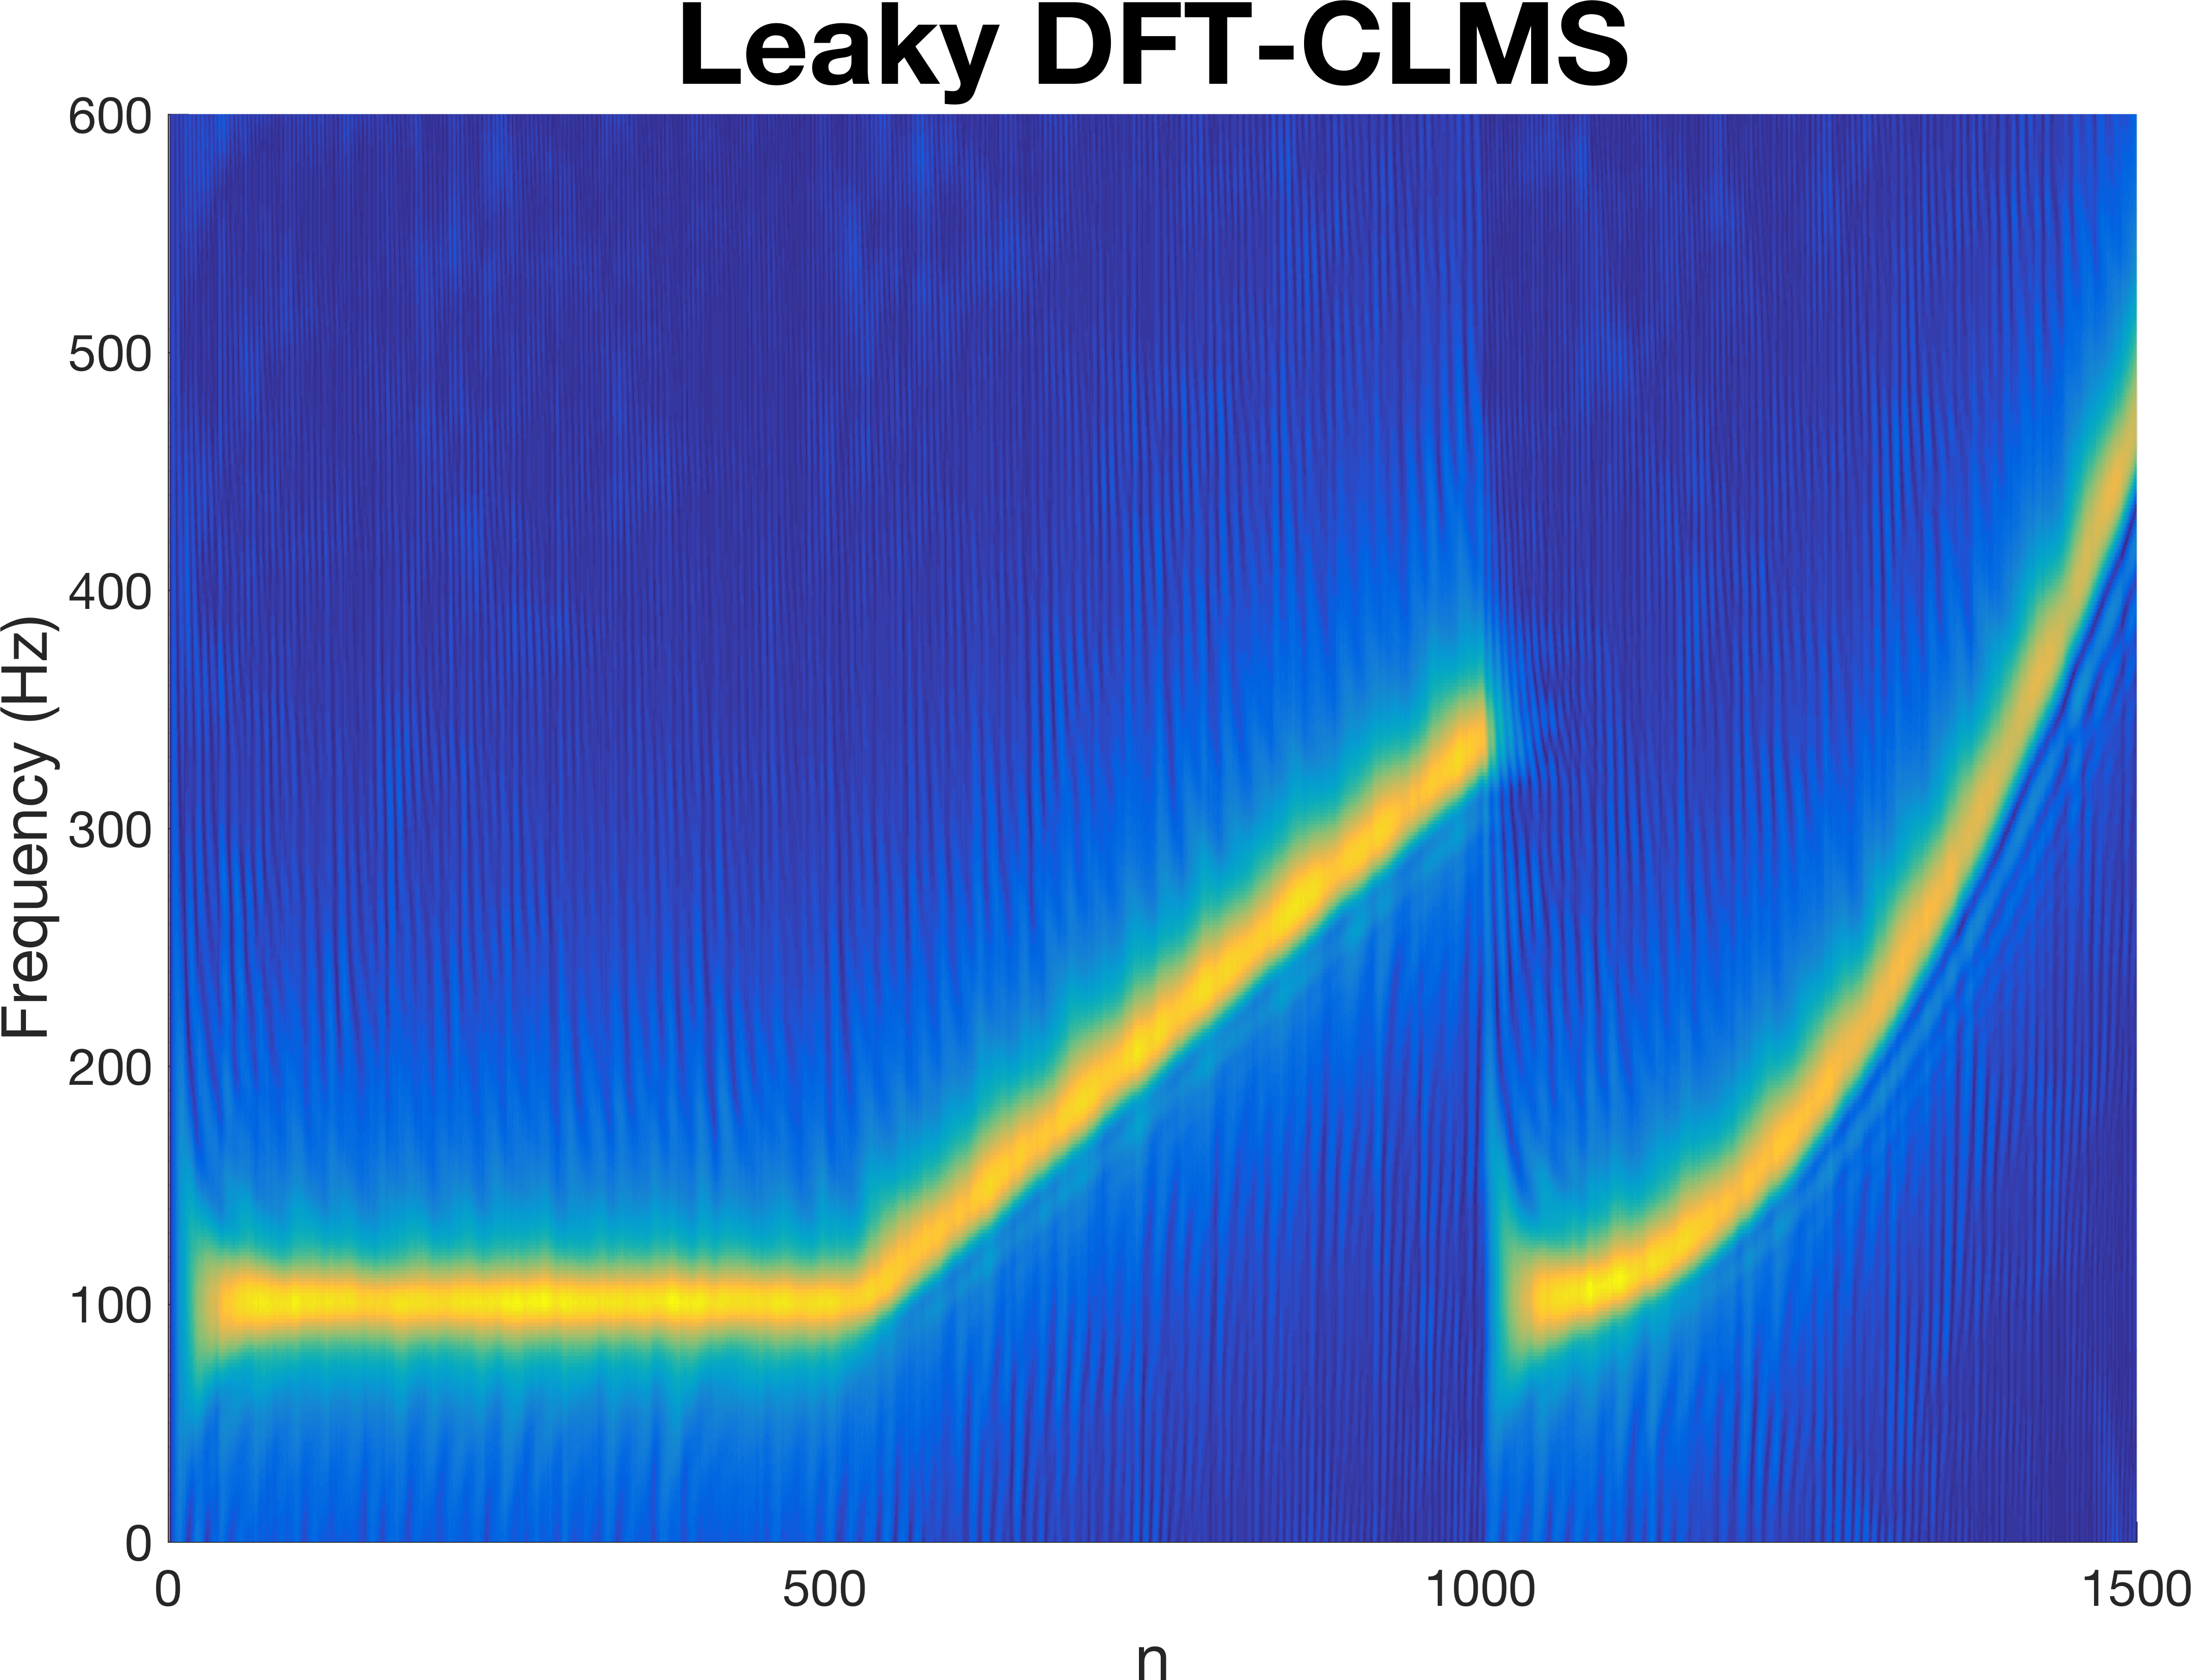
\includegraphics[width=0.32\textwidth]{part4/time_frequency_dft_leaky}
\caption{Time-Frequency Estimation using DFT-CLMS and Leaky DFT-CLMS}
\end{figure}

\begin{figure}[H]
\centering{}
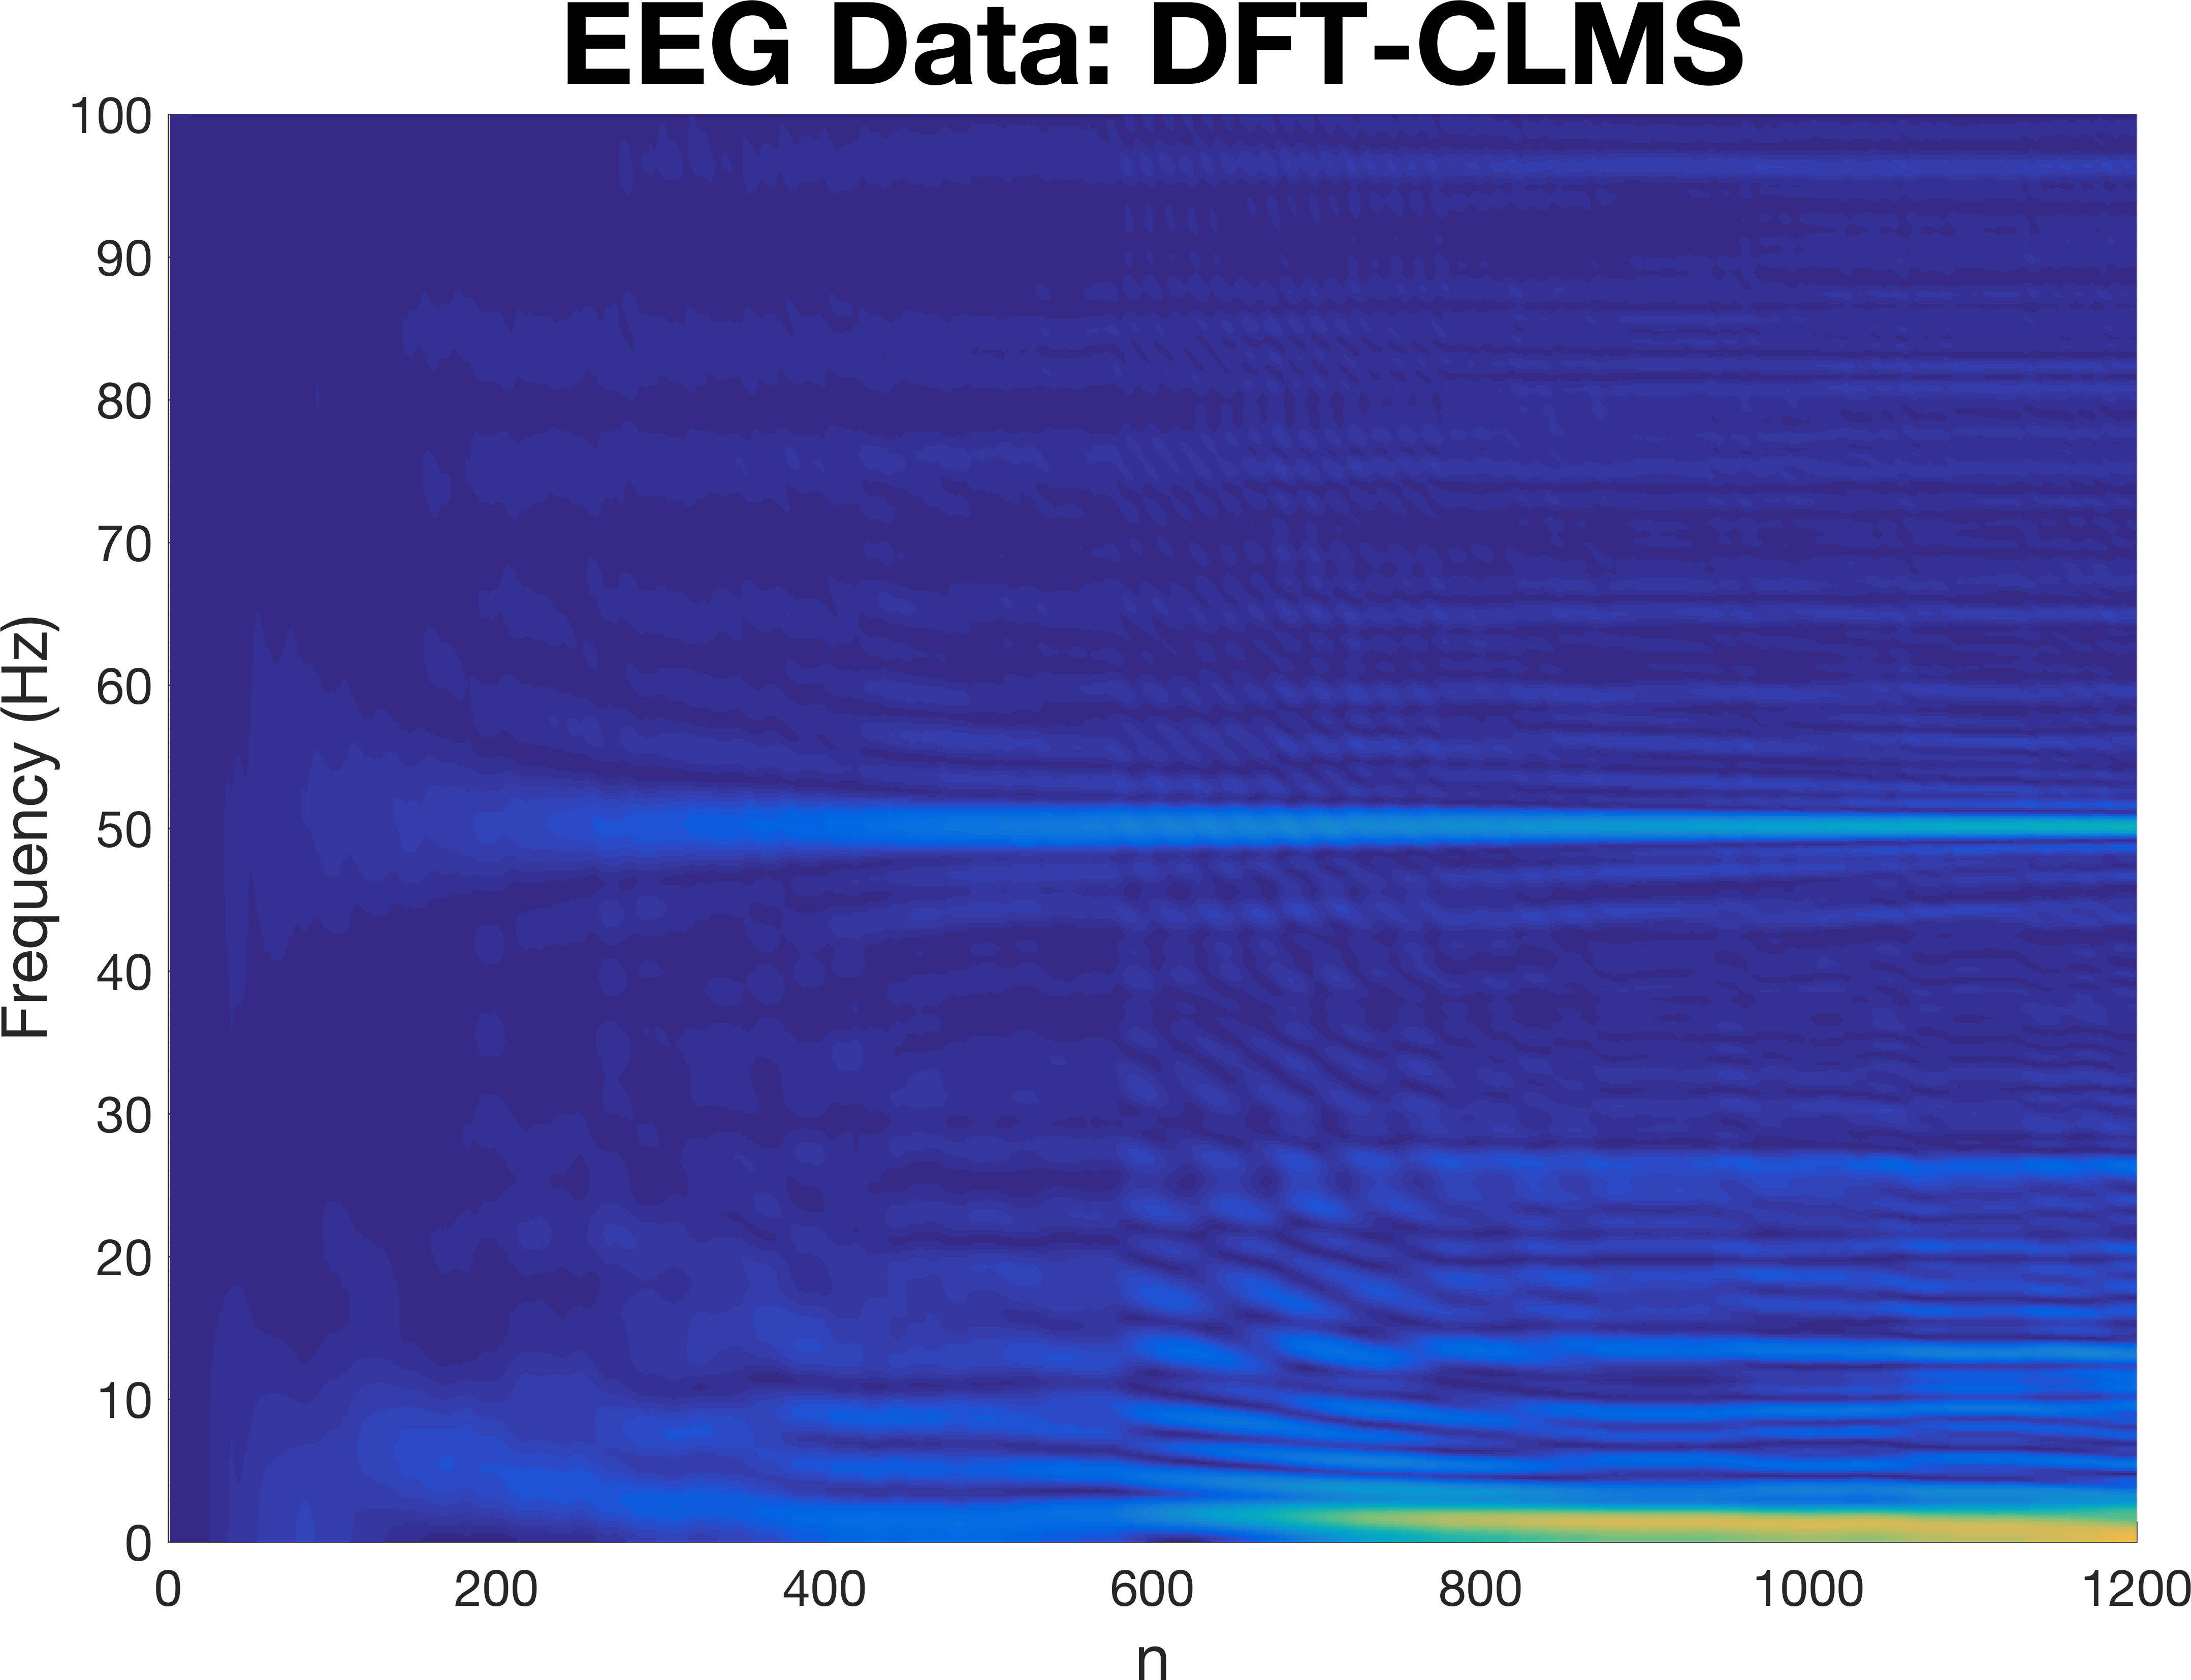
\includegraphics[width=0.32\textwidth]{part4/eeg_time_frequency_dft_non_leaky}
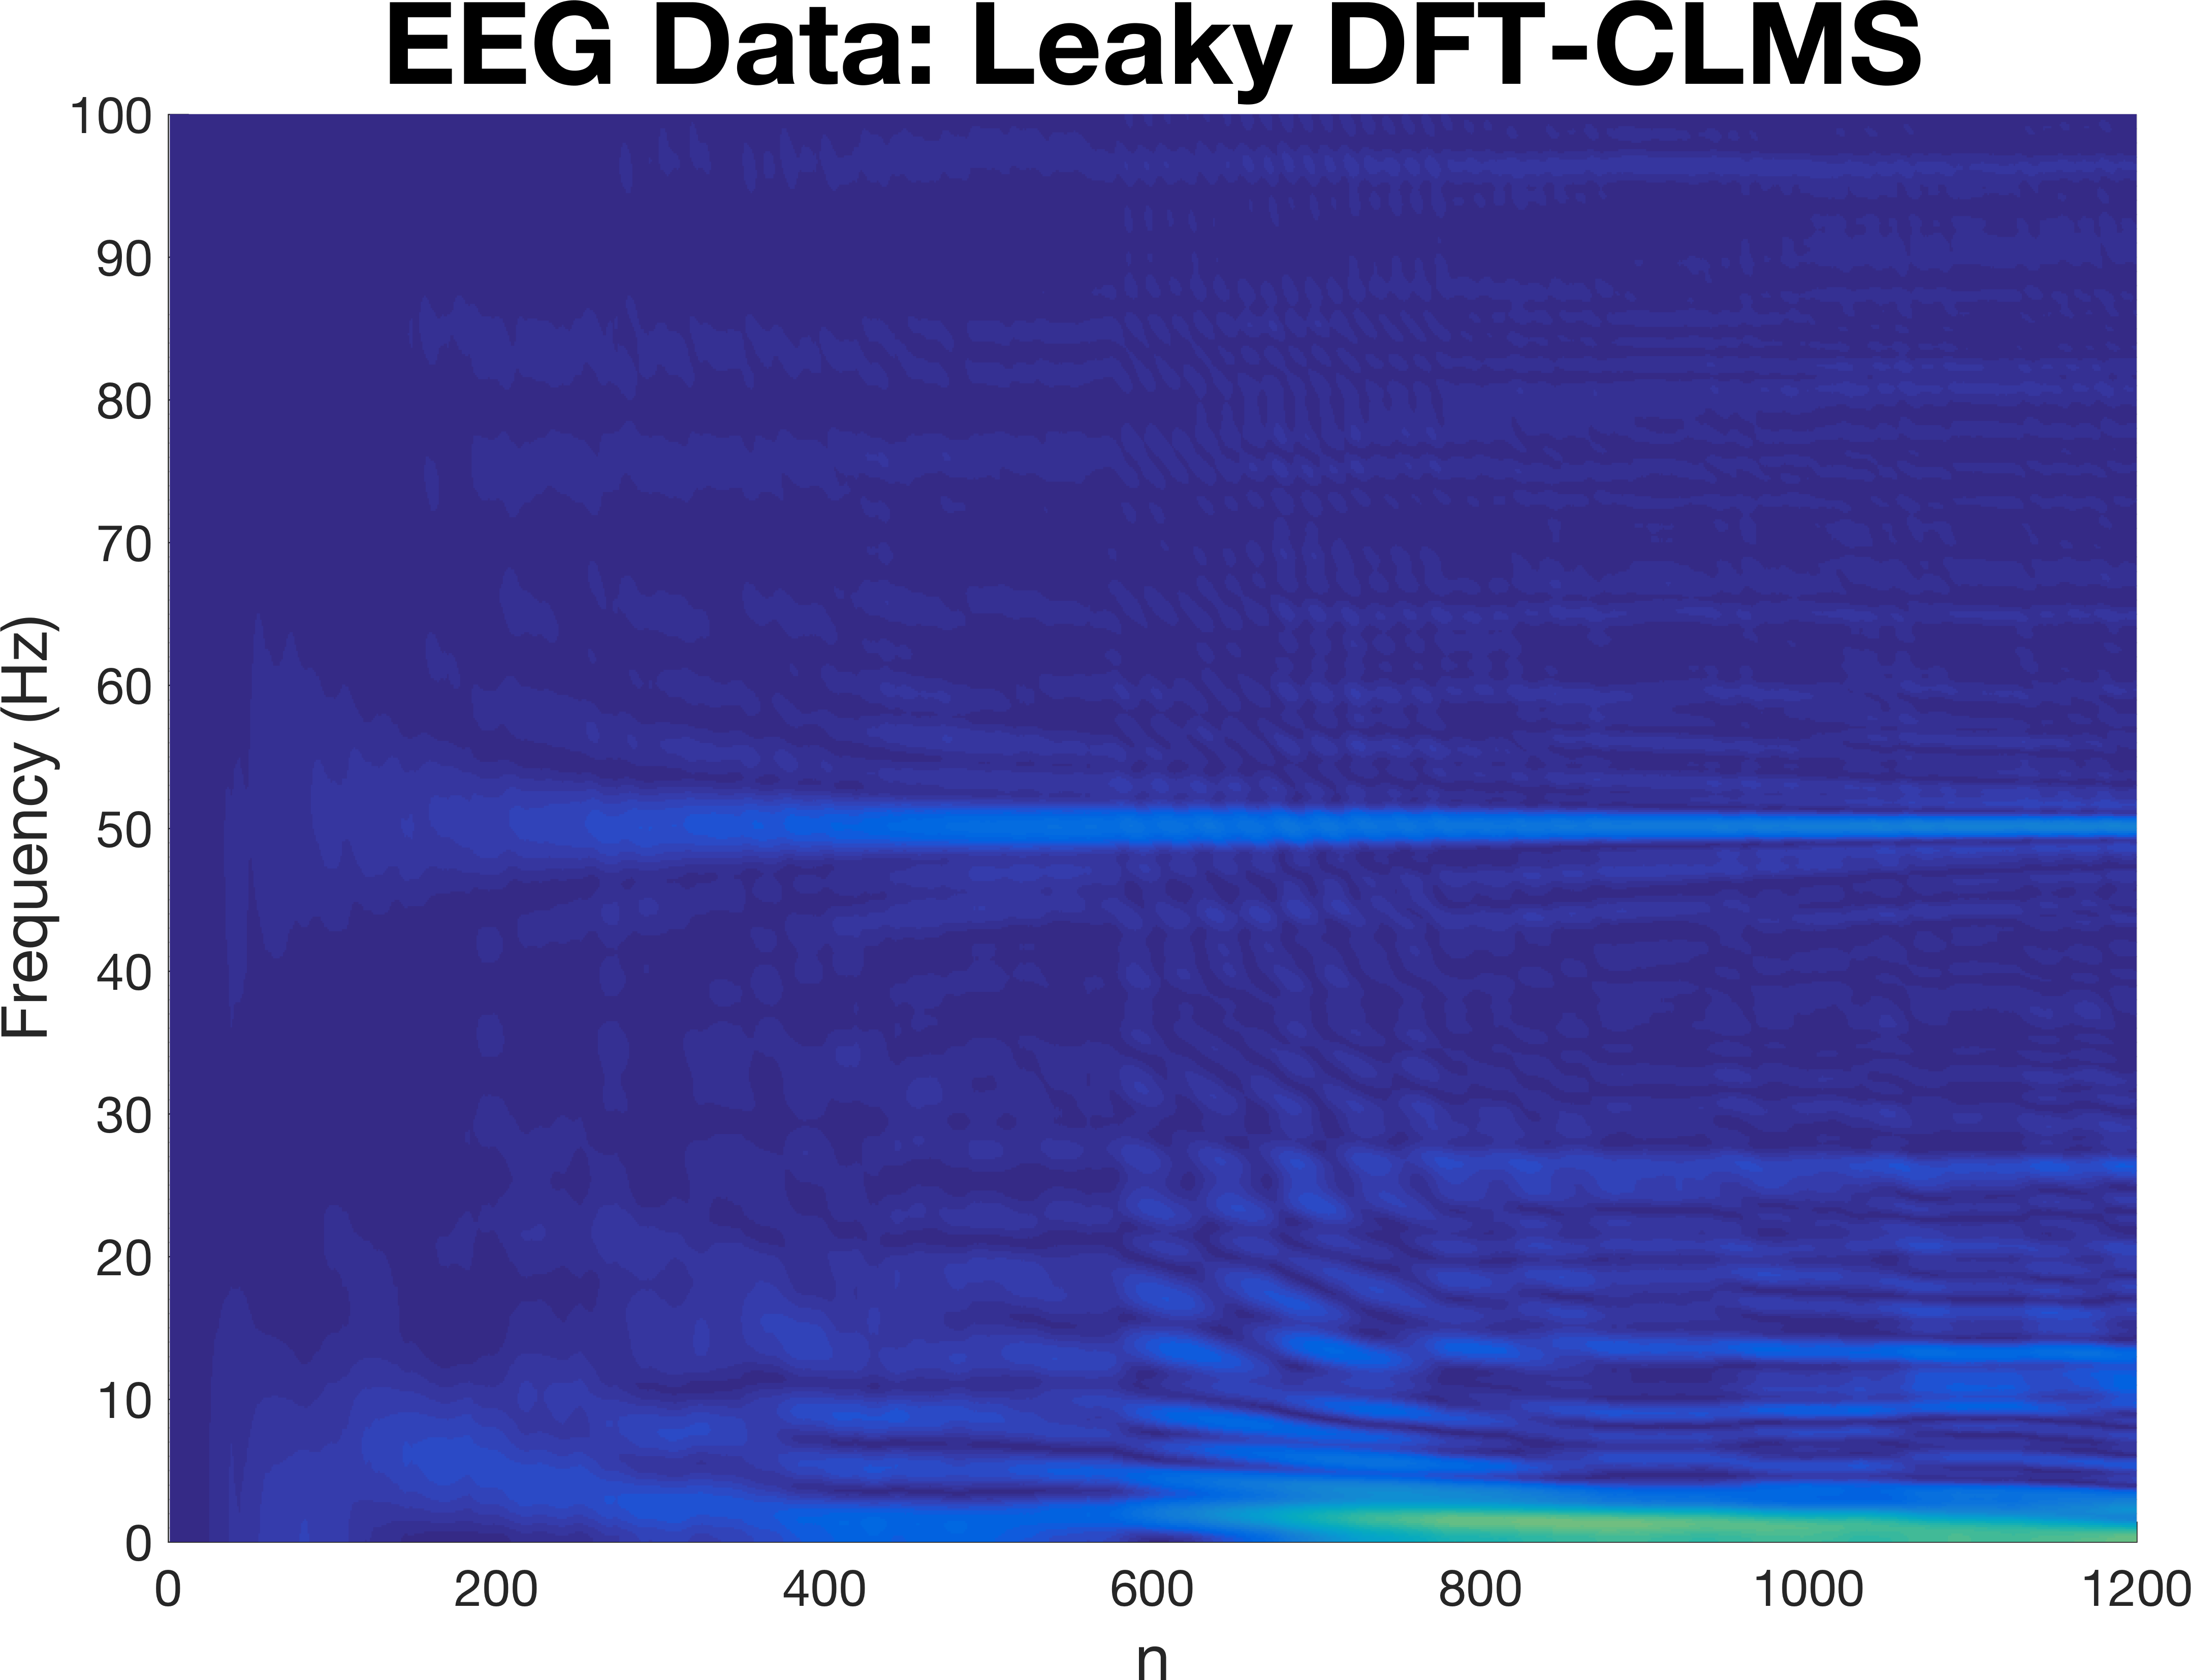
\includegraphics[width=0.32\textwidth]{part4/eeg_time_frequency_dft_leaky}
\caption{}
\end{figure}





